\g
\chapter{Υλοποίηση - Πειραματικό Μέρος}
\label{Chapter4}
%%%%%%%%%%%%%%%%%%%%%%%%%%%%%%%%%%%%%%%%%%%%%%%%%%%%%%%%%%%%%%%%%%%%%%%%%%
\section{Υπολογιστικό Σύστημα}

Τα πειράματα υλοποιήθηκαν σε σταθερό υπολογιστή με τα εξής χαρακτηριστικά:

\begin{itemize}
	\item \textbf{Λειτουργικό σύστημα:} \e Linux Ubuntu 16.04 \g
	\item \textbf{Επεξεργαστής:} \e 4x Intel® Core™ i5-4690 CPU @ 3.50 GHz (6M Cache) \g
	\item \textbf{Μνήμη \e RAM\g:} \e DDR3 16GB\g
	\item \textbf{Κάρτα γραφικών:} \e NVIDIA GeForce GTX 1060 (memory: 6GB, clock: 1.5 GHz, bandwidth: $192\dfrac{GB}{s}$, CUDA cores:1280) \g
\end{itemize}

Όλα τα πειράματα υλοποιήθηκαν σε περιβάλλον \e Python. \g Σε συγκεκριμένες περιπτώσεις για την επιτάχυνση των αλγορίθμων αξιοποιήθηκε ο στατικός μεταγλωτιστής \e Cython. \g Χρησιμοποιήθηκαν επίσης οι βιβλιοθήκες:

\begin{itemize}
	\item \e tensorflow \g
	\item \e numpy \g
	\item \e matplotlib \g
	\item \e opencv \g
\end{itemize}

%%%%%%%%%%%%%%%%%%%%%%%%%%%%%%%%%%%%%%%%%%%%%%%%%%%%%%%%%%%%%%%%%%%%%%%%
\section{Εκπαίδευση νευρωνικoύ δικτύου}

Εκπαιδεύουμε το νευρωνικό δίκτυο σε εγγραφές που εξάγουμε αποκλειστικά από το σετ δεδομένων \e KITTI 2012 \g που περιέχει συνολικά 194 εικόνες αφού το διαχωρίσουμε σε σετ εκπαίδευσης και σετ επικύρωσης, με συντελεστή αναλογίας $\mathtt{pcg\_tr} = 0.6$. Επομένως, χρησιμοποιούνται $\mathbf{int}(\mathtt{pcg\_tr} \times 194) = 116$ εικόνες για την εκπαίδευση και $\mathbf{int}((1-\mathtt{pcg\_tr}) \times 194) = 78$ για την επικύρωση. Κάθε δέσμη \e (batch) \g εκπαίδευσης περιέχει $\mathtt{batch\_size} = 128$ εγγραφές που αναλογούν σε τυχαίες θέσεις εντός της εικόνας επιδιώκοντας την μικρότερη δυνατή συσχέτιση των παραδειγμάτων εντός της ίδιας δέσμης. Ορίζουμε ανώτατο όριο \e batches \g ανά εικόνα $\mathtt{batches\_limit} = 40$, για να εξασφαλίσουμε μικρή συσχέτιση μεταξύ τους. Με αυτήν την μεθοδολογία:
\begin{itemize}
	\item από κάθε εικόνα εξάγονται $\mathtt{batches\_limit}\times\mathtt{batch\_size} = 5120$ παραδείγματα.
	\item κάθε εποχή εκπαίδευσης \e (training epoch) \g περιέχει $$\mathbf{int}(195 \times \mathtt{pcg\_tr}) \times \mathtt{batches\_limit} = 4640 \: \text{δέσμες}$$ που αναλογούν σε $$\mathbf{int}(195 \times \mathtt{pcg\_tr}) \times \mathtt{batches\_limit} \times \mathtt{batch\_size} = 593920 \: \text{παραδείγματα.}$$
\end{itemize}

Κατά την εκπαίδευση, σε κάθε μπλοκ \e conv2d + BN + ReLU \g προσθέτουμε ένα επίπεδο \e dropout \citep{JMLR:v15:srivastava14a} \g με ποσοστό αποκοπής νευρώνων $40\%$.

Χρησιμοποιούμε τον βελτιστοποιητή \e (optimizer) ADAM \citep{kingma2014adam} \g  με αρχικό βαθμό εκμάθησης \e (learning rate) \g $0.01$. Μειώνουμε τον βαθμό εκμάθησης κατά τον παράγοντα $5$ κάθε $6000$ επαναλήψεις εκπαίδευσης, από την επανάληψη $20000$ και μετά.

Παρακολουθούμε τη μεταβολή του κόστους εντροπίας \ref{fig:xentropy} σε κάθε βήμα εκπαίδευσης και ελέγχουμε το απόλυτο σφάλμα πρόβλεψης και το απόλυτο σφάλμα πρόβλεψης με ανώφλι κάθε $1000$ βήματα εκπαίδευσης\footnote{Για λόγους ταχύτητας, τα απόλυτα σφάλματα υπολογίζονται στις μισές εικόνες εκπαίδευσης κι επικύρωσης της συλλογής.} \ref{fig:error_during_training}. Παρατηρούμε ότι οι καμπύλες σφάλματος και απόκλισης μεταξύ του σετ εκπαίδευσης και του σετ επικύρωσης εμφανίζουν πολύ μεγάλη ομοιότητα, σχεδόν ταύτιση, επιβεβαιώνοντας ότι το δίκτυο δεν έχει υποστεί υπερπροσαρμογή \e (overfitting). \g Από τις καμπύλες παρατηρούμε ότι η εκπαίδευση τελματώνεται μετά από περίπου $20000$ επαναλήψεις. Επιλέγουμε να κρατήσουμε τις τιμές όλων των εκπαιδεύσιμων παραμέτρων κατά το βήμα $25000$.\footnote{Κατά την εκπαίδευση αποθηκεύονται όλες οι εκπαιδεύσιμες παράμετροι του δικτύου κάθε $1000$ επαναλήψεις.} Η εκπαίδευση διήρκεσε συνολικά περίπου $7$ ώρες.

\begin{figure}
	\centering
	\begin{subfigure}{\textwidth}
		\centering
		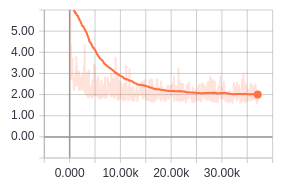
\includegraphics[width=0.6\textwidth]{xentropy_mean_loss_over_batch.png}
		\caption{Μέσο κόστος εντροπίας ανά δέσμη κατά την διάρκεια της εκπαίδευσης.}
	\end{subfigure}
	\begin{subfigure}{\textwidth}
		\centering
		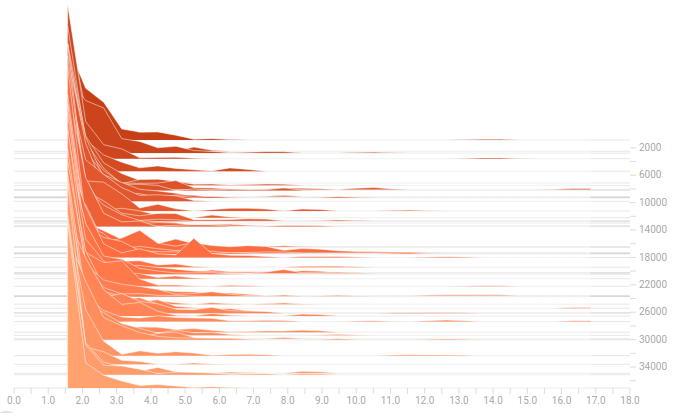
\includegraphics[width=0.6\textwidth]{xentropy_loss_per_batch.png}
		\caption{Ιστόγραμμα κόστους εντροπίας για κάθε παράδειγμα της δέσμης εκπαίδευσης κατά την διάρκεια όλης της εκπαίδευσης.}
	\end{subfigure}
	
	\caption{Η μείωση του κόστους εντροπίας είναι ικανοποιητική μέχρι το βήμα $20000$. Από εκεί και πέρα η βελτίωση του δικτύου είναι ισχνή.}
	\label{fig:xentropy}
\end{figure}

\begin{figure}
	\centering
	\begin{subfigure}{\textwidth}
		\centering
		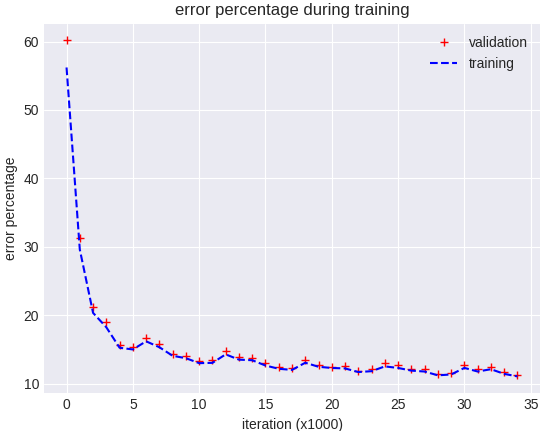
\includegraphics[width=0.8\textwidth]{error_during_training.png}
		\caption{Εξέλιξη μέσου απόλυτου σφάλματος με κατώφλι κατά την διάρκεια της εκπαίδευσης.}
	\end{subfigure}
	\begin{subfigure}{\textwidth}
		\centering
		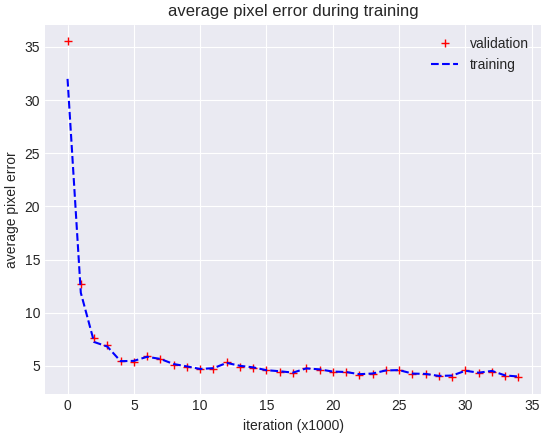
\includegraphics[width=0.8\textwidth]{error_mean_during_training.png}
		\caption{Εξέλιξη μέση απόλυτου σφάλματος κατά την διάρκεια της εκπαίδευσης.}
	\end{subfigure}
	
	\caption{Παρατηρούμε και στα δύο γραφήματα οι καμπύλες που αναλογούν στο σετ εκπαίδευσης και επικύρωσης σχεδόν ταυτίζονται, φαινόμενο που αποτελεί έντονη ένδειξη ότι το δίκτυο δεν έχει υποστεί υπερπροσαρμογή. Τα γραφήματα επιβεβαιώνουν ότι η βελτίωση μετά το βήμα εκπαίδευσης $20000$ είναι ανεπαίσθητη.}
	\label{fig:error_during_training}
\end{figure}

\begin{figure}
	\centering
	\begin{subfigure}{0.45\textwidth}
		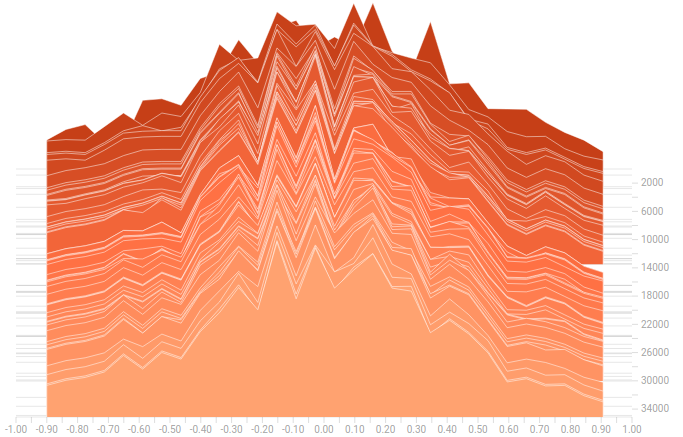
\includegraphics[width=\textwidth]{weights_layer_1.png}
		\caption{Ιστόγραμμα βαρών του πρώτου επιπέδου.}
	\end{subfigure}
	\begin{subfigure}{0.45\textwidth}
		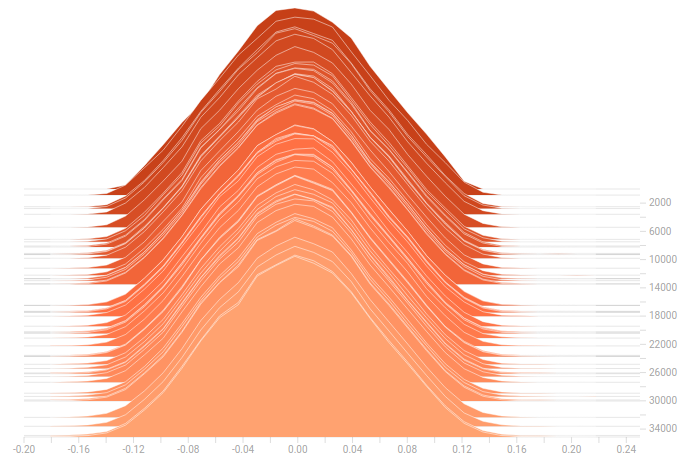
\includegraphics[width=\textwidth]{weigths_layer_4.png}
		\caption{Ιστόγραμμα βαρών του τέταρτου επιπέδου.}
	\end{subfigure}
	
	\begin{subfigure}{0.45\textwidth}
		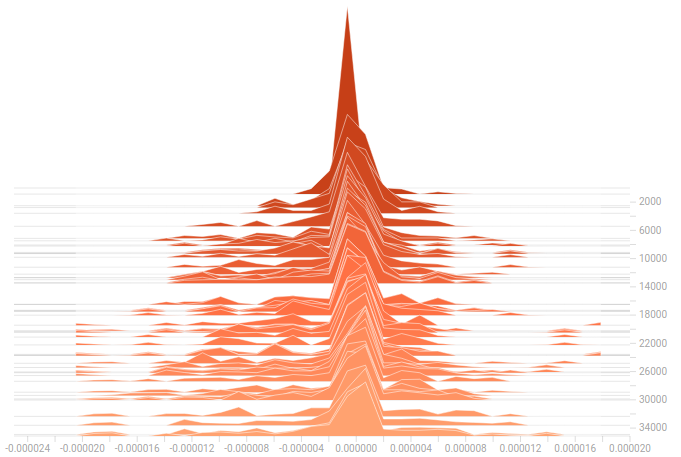
\includegraphics[width=\textwidth]{biases_layer_1.png}
		\caption{Ιστόγραμμα πολώσεων πρώτου επιπέδου.}
	\end{subfigure}
	\begin{subfigure}{0.45\textwidth}
		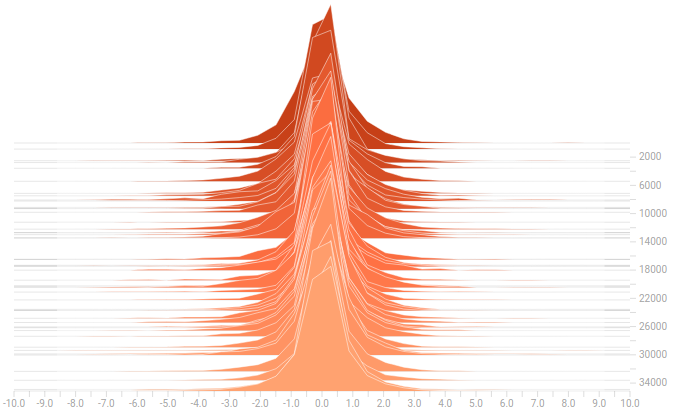
\includegraphics[width=\textwidth]{pre_bn_layer_1.png}
		\caption{Ιστόγραμμα εξόδου συνέλιξης πρώτου επιπέδου.}
	\end{subfigure}
	
	\begin{subfigure}{0.45\textwidth}
		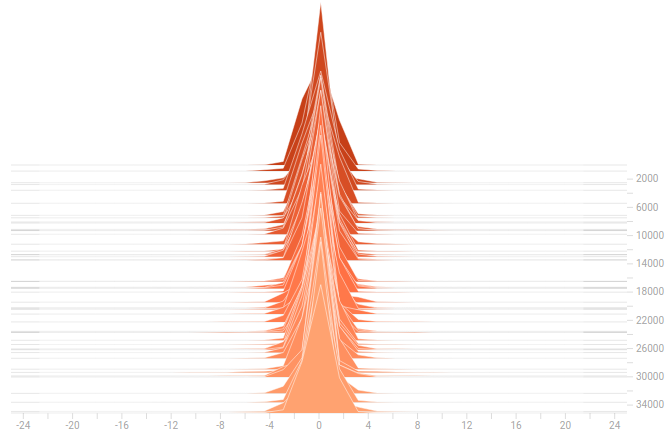
\includegraphics[width=\textwidth]{after_bn_layer_1.png}
		\caption{Ιστόγραμμα εξόδου επιπέδου \e batch normalization. \g}
	\end{subfigure}
	\begin{subfigure}{0.45\textwidth}
		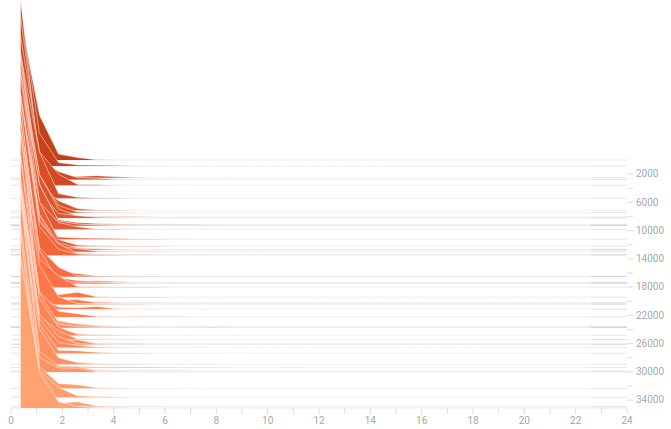
\includegraphics[width=\textwidth]{after_ReLU_layer_1.png}
		\caption{Ιστόγραμμα εξόδου συνάρτησης ενεργοποίησης \e ReLU. \g}
	\end{subfigure}
	
	\caption{Παρατηρήσεις: \e(i) \g Η κατανομή των βαρών δεν είναι όμοια σε όλα τα επίπεδα. Όπως φαίνεται στην εικόνα (Α') τα βάρη του πρώτου επιπέδου δεν ακολουθούν απόλυτα κανονική κατανομή και κυμαίνονται στο διάστημα $[-0.8,0.8]$, ενώ αυτά του τέταρτου επιπέδου ακολουθούν απόλυτα κανονική και κυμαίνονται στο διάστημα $[-0.15,0.15]$. \e(ii) \g Οι πολώσεις του πρώτου επιπέδου (σχήμα (Β')), όπως και των υπόλοιπων επιπέδων είναι τάξης μεγέθους $10^{-5}$. Ουσιαστικά το δίκτυο δεν χρειάζεται τον αφινικό μετασχηματισμό \e $y=\mathbf(conv2d(x,h)) + b$ \g και τον περιορίζει στον γραμμικό $y=\mathbf(conv2d(x,h))$. Το φαινόμενο αυτό παρουσιάζεται συχνά όταν ακολούθως χρησιμοποιείται επίπεδο κανονικοποίησης δέσμης.\e(iii) \g Στα σχήματα (Δ'),(Ε'),(ΣΤ') οι τιμές βρίσκονται εντός των διαστημάτων $[-7,7]$, $[-7,7]$ και $[0,7]$ αντίστοιχα.}
	\label{fig:layer_histograms}
\end{figure}


%%%%%%%%%%%%%%%%%%%%%%%%%%%%%%%%%%%%%%%%%%%%%%%%%%%%%%%%%%%%%%%%%%%%%%%%
\section{Αρχικοποίηση κόστους αντιστοίχησης}

Σε κάθε μια από τις παρακάτω ενότητες, υπολογίζουμε τον πίνακα κόστους $C$ με τους υπό δοκιμή αλγορίθμους και ακολούθως υπολογίζουμε τον χάρτη παράλλαξης, εφαρμόζοντας την πράξη $D(\mathbf{p}) = \mathbf{arg\_min}_d(\mathbf{p})$. Επιλέγουμε τυχαία το στερεοσκοπικό ζεύγος $4$ της συλλογής \e KITTI 2012 \g για την οπτικοποίηση των αποτελεσμάτων.

%%%%%%%%%%%%%%%%%%%%%%%%%%%%%%%%%%%%%%%%%%%%%%%%%%%%%%%%%%%%%%%%%%%%%%%
\subsection{Συμβατικές μέθοδοι}

\subsubsection{Άθροισμα απόλυτων διαφορών}

Όπως είδαμε στο κεφάλαιο 2 είναι δύσκολη η επιλογή περιοχής άθροισης κατάλληλου μεγέθους. Όσο μεγαλώνει, τόσο ο χάρτης εμφανίζεται πιο λείος αλλά με θολωμένες τις ακμές, ενώ αντίθετα όσο μικραίνει τόσο αυξάνεται η λεπτομέρεια στις ακμές με κόστος πολλές εξωκείμενες τιμές. Στο σχήμα \ref{fig:SAD_multiple_windows} απεικονίζεται το παραπάνω φαινόμενο. Η καλύτερη επίδοση στο παράδειγμά εμφανίζεται για μέγεθος παραθύρου $\mathtt{window\_size} = 21\:px$ με ποσοστό απόλυτου σφάλματος $16.7\%$.

\begin{figure}
	\centering
	\begin{subfigure}{0.32\textwidth}
		\caption{$I^L$}
		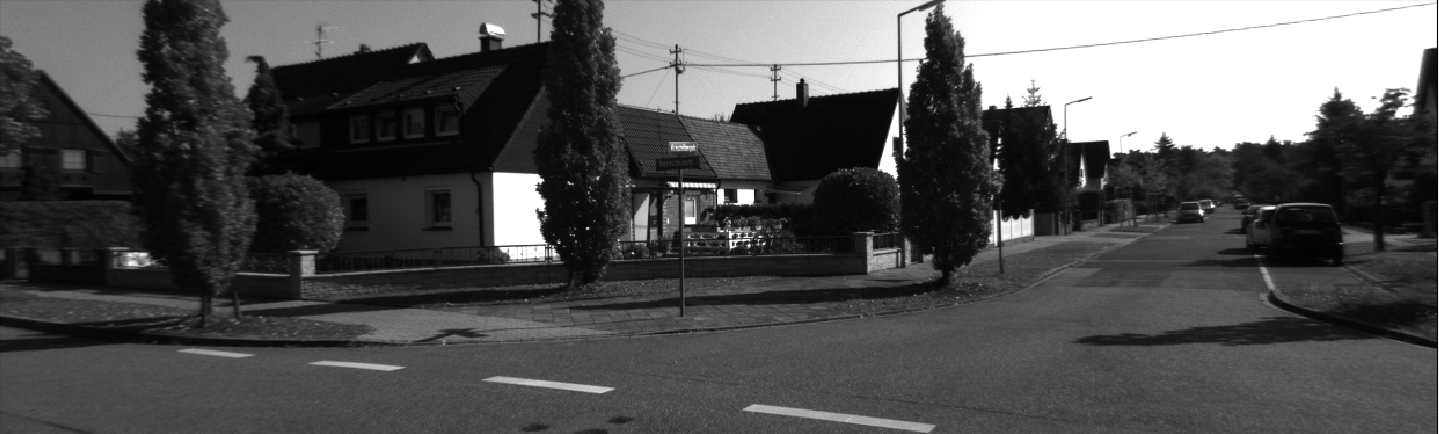
\includegraphics[width=\textwidth]{im4_imL.png}
	\end{subfigure}
	\begin{subfigure}{0.32\textwidth}
		\caption{$I^R$}
		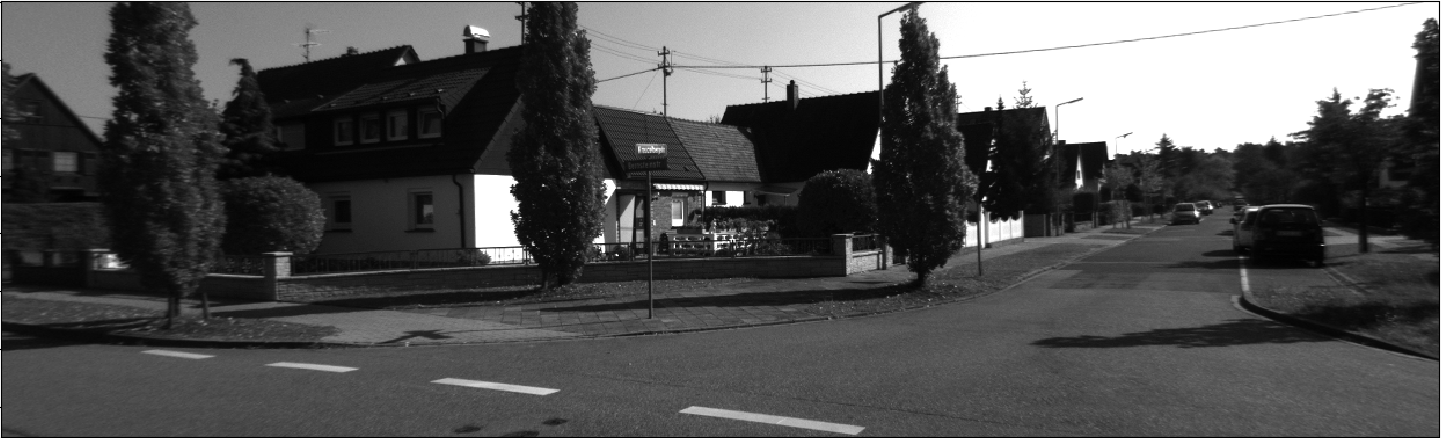
\includegraphics[width=\textwidth]{im4_imR.png}
	\end{subfigure}
	\begin{subfigure}{0.32\textwidth}
		\caption{\e $\mathbf{ground\_trouth}$ \g}
		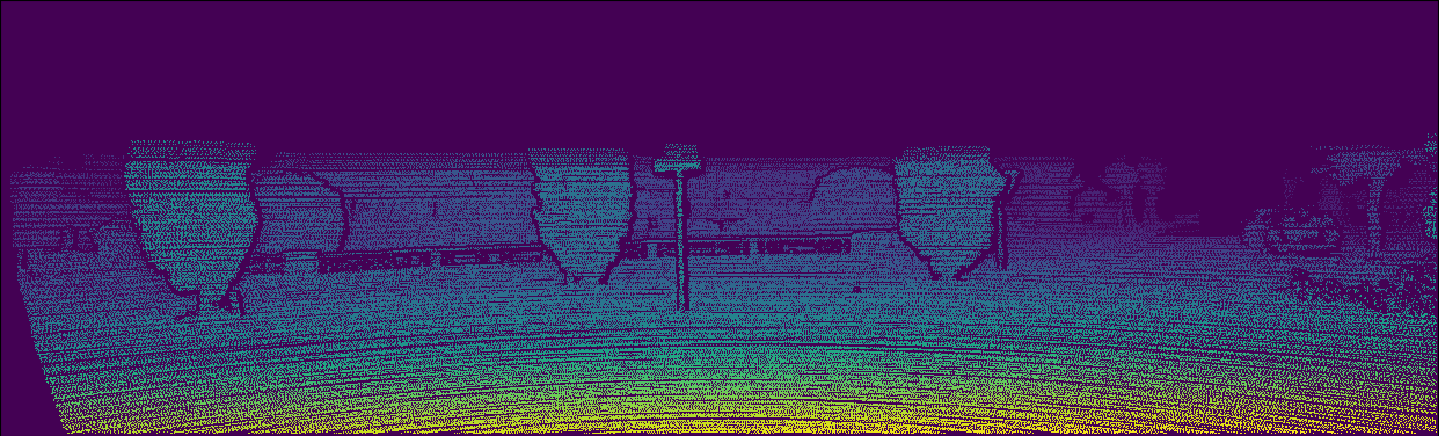
\includegraphics[width=\textwidth]{im4_disp_gt.png}
	\end{subfigure}

	\begin{subfigure}{0.45\textwidth}
		\caption{\e $\mathbf{window = 9 px}$ \g}
		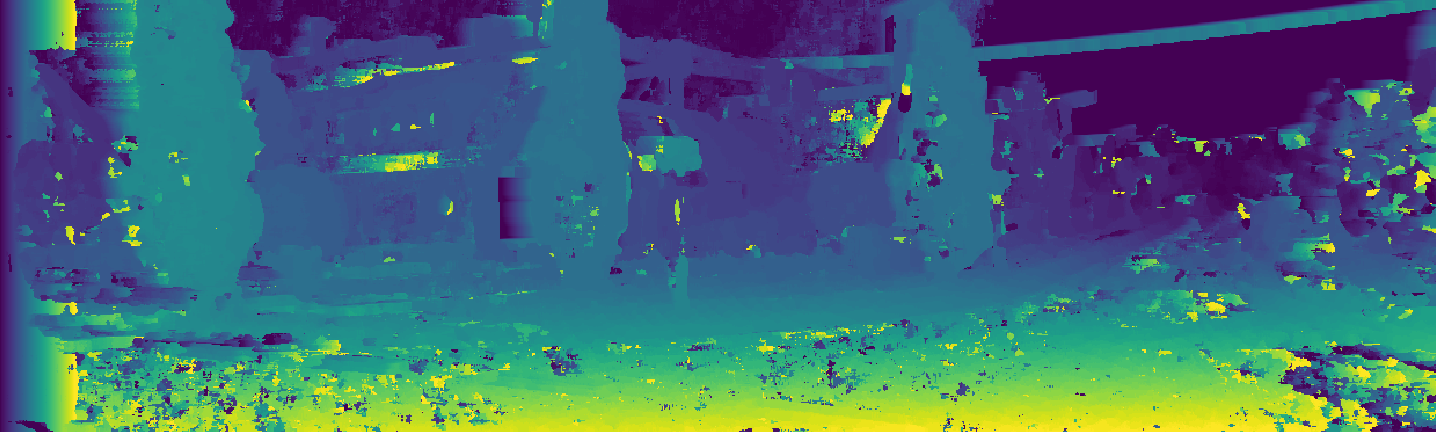
\includegraphics[width=\textwidth]{SAD_win_9.png}
	\end{subfigure}
	
	\begin{subfigure}{0.45\textwidth}
		\caption{\e $\mathbf{window = 15 px}$ \g}
		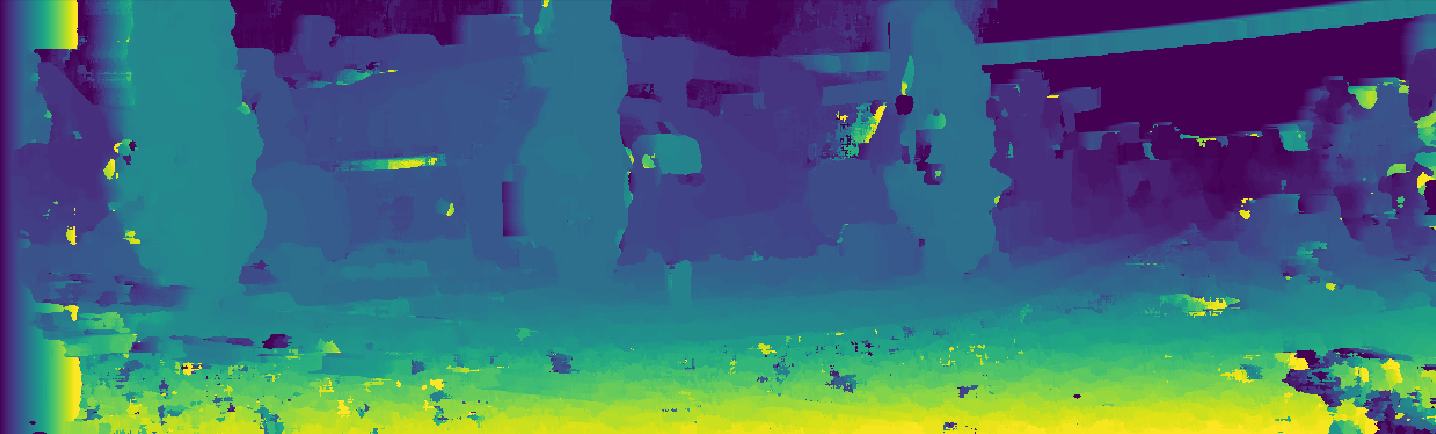
\includegraphics[width=\textwidth]{SAD_win_15.png}
	\end{subfigure}
	
	\begin{subfigure}{0.45\textwidth}
		\caption{\e $\mathbf{window = 21 px}$ \g}
		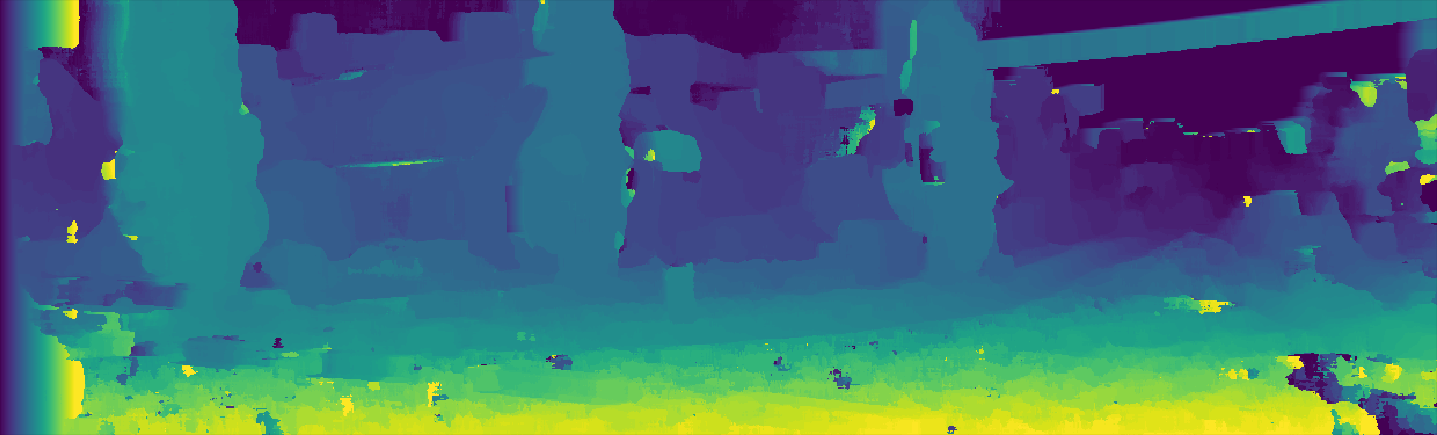
\includegraphics[width=\textwidth]{SAD_win_21.png}
	\end{subfigure}
		\begin{subfigure}{0.45\textwidth}
		\caption{\e Error: $16.7\%$ \g}
		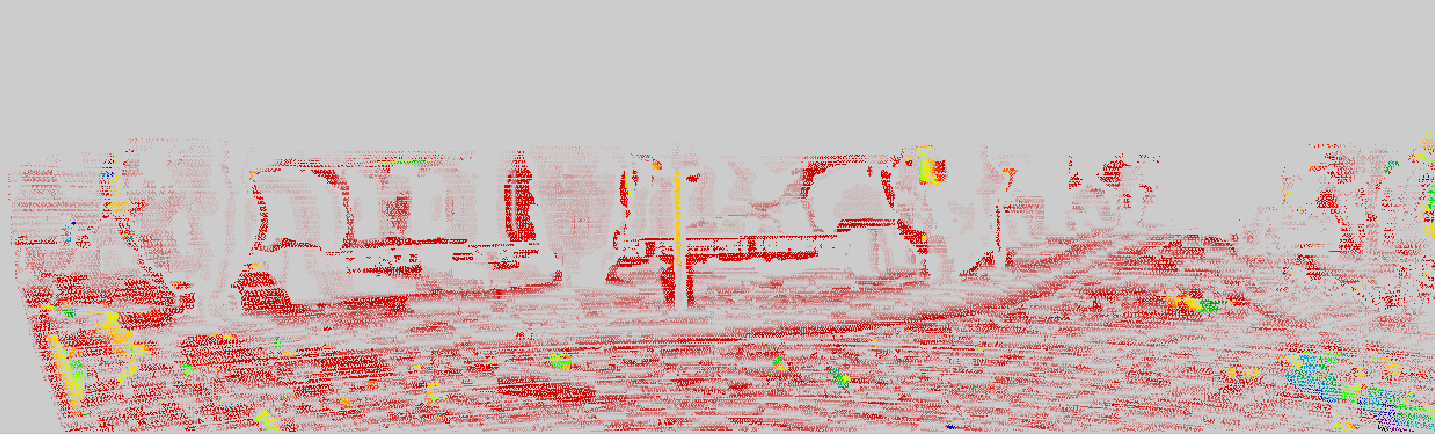
\includegraphics[width=\textwidth]{SAD_win_21_err.png}
	\end{subfigure}
	
	\begin{subfigure}{0.45\textwidth}
		\caption{\e $\mathbf{window = 27 px}$ \g}
		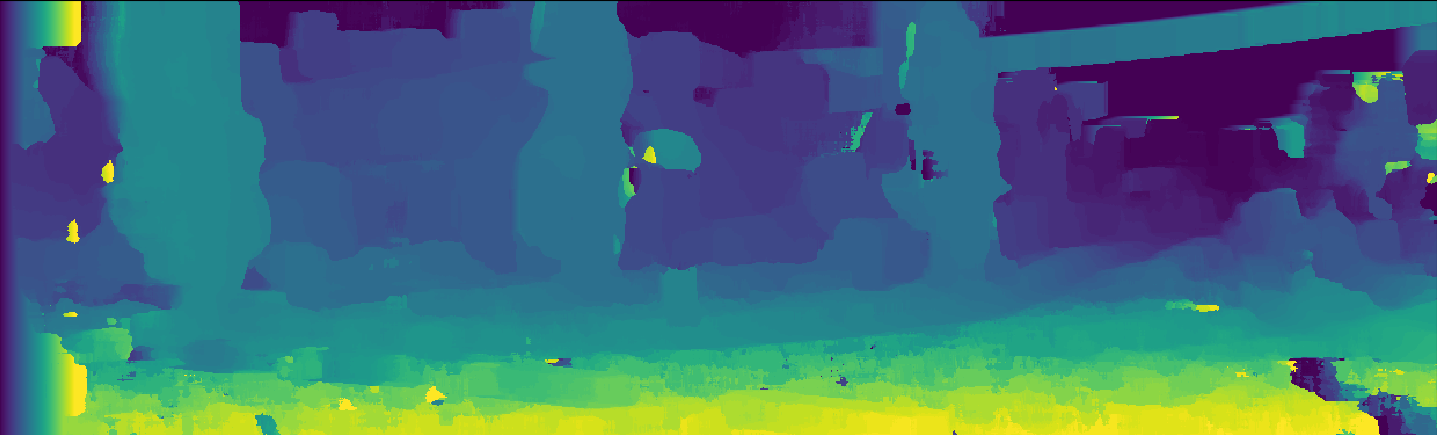
\includegraphics[width=\textwidth]{SAD_win_27.png}
	\end{subfigure}
	
	\begin{subfigure}{0.45\textwidth}
		\caption{\e $\mathbf{window = 33 px}$ \g}
		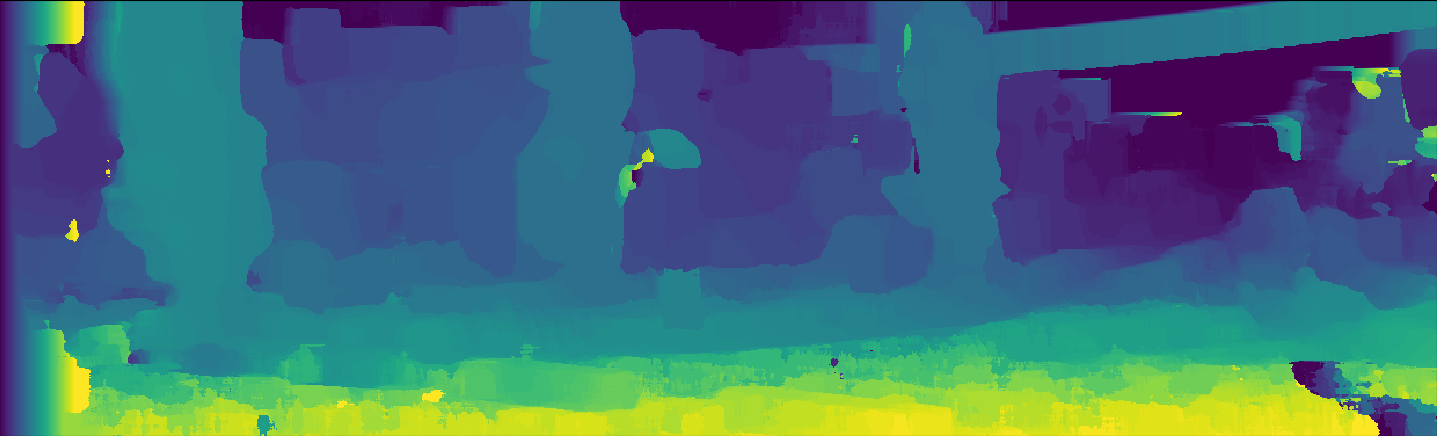
\includegraphics[width=\textwidth]{SAD_win_33.png}
	\end{subfigure}
	
	\begin{subfigure}{0.45\textwidth}
		\caption{\e $\mathbf{window = 39 px}$ \g}
		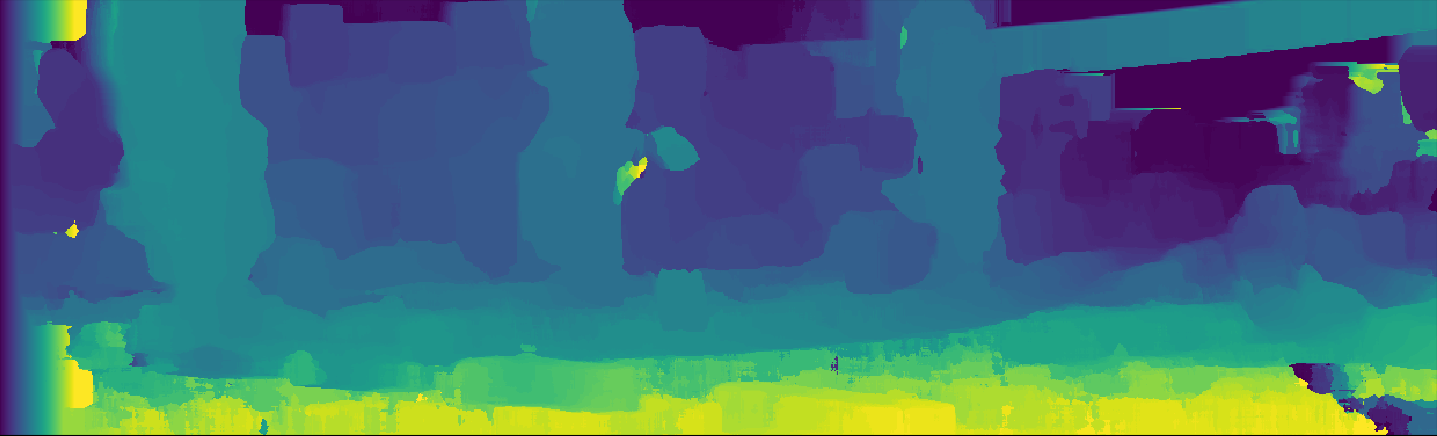
\includegraphics[width=\textwidth]{SAD_win_39.png}
	\end{subfigure}
	
	\caption{Άθροισμα απόλυτων διαφορών σε παράθυρα διαφορετικού μεγέθους.}
	\label{fig:SAD_multiple_windows}
\end{figure}

\subsubsection{Μετασχηματισμός \texorpdfstring{\e Census\g}{TEXT}}

O μετασχηματισμός \e census \citep{zabih1994non} \g δημιουργεί τοπικό περιγραφέα που είναι ανεπηρέαστος από τις φωτομετρικές αποκλίσεις. Ταυτόχρονα όμως έχει το μειονέκτημα να δημιουργεί παρόμοιο περιγραφέα από τελείως διαφορετικά είδωλα που τυχαίνει να δημιουργούν γειτονιές με παρόμοια σχέση φωτεινότητας περιφέρειας και κεντρικού \e pixel. \g Στο σχήμα \ref{fig:census_multiple_windows} αποτυπώνεται αυτό το φαινόμενο καθώς οι υπολογισμένοι χάρτες παράλλαξης εμφανίζουν έντονες ασυνέχειες. Βέλτιστη επίδοση εμφανίζει για μέγεθος παραθύρου $\mathtt{window\_size} = 27\:px$ με ποσοστό απόλυτου σφάλματος $32.27\%$.

\begin{figure}
	\centering
	\begin{subfigure}{0.32\textwidth}
		\caption{$I^L$}
		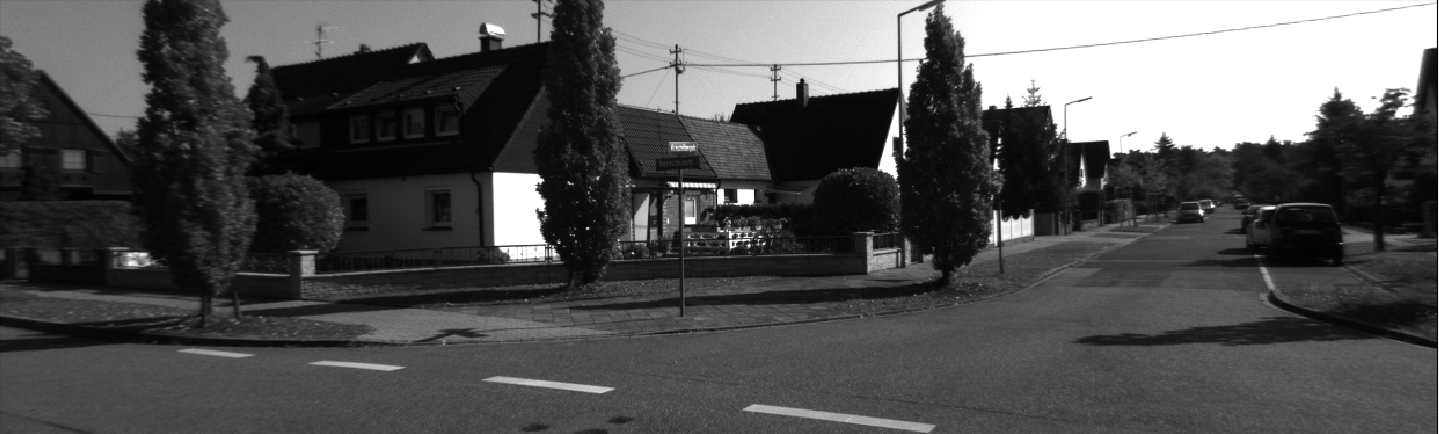
\includegraphics[width=\textwidth]{im4_imL.png}
	\end{subfigure}
	\begin{subfigure}{0.32\textwidth}
		\caption{$I^R$}
		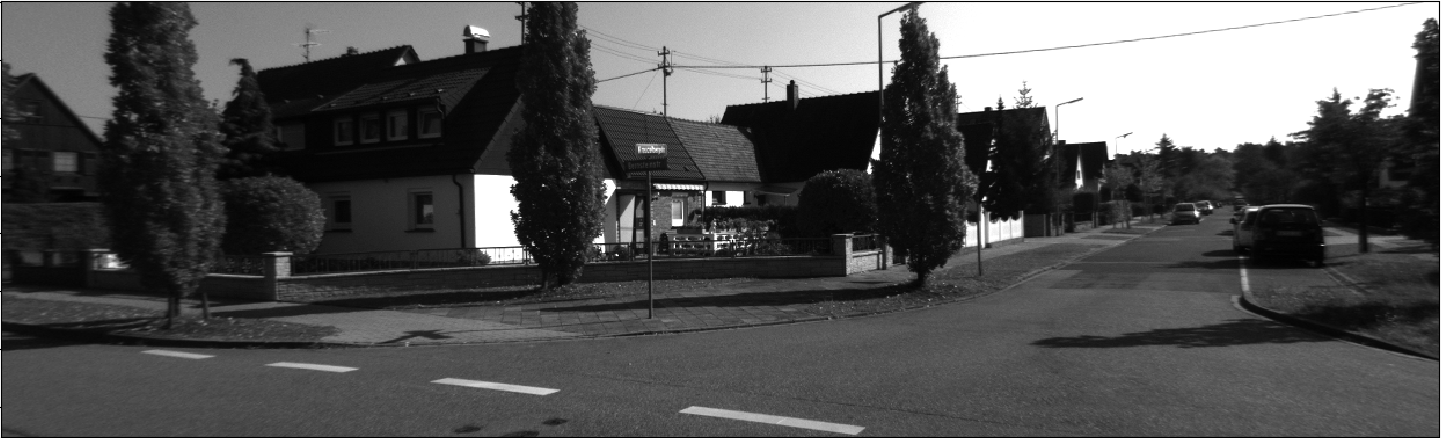
\includegraphics[width=\textwidth]{im4_imR.png}
	\end{subfigure}
	\begin{subfigure}{0.32\textwidth}
		\caption{\e $\mathbf{ground\_trouth}$ \g}
		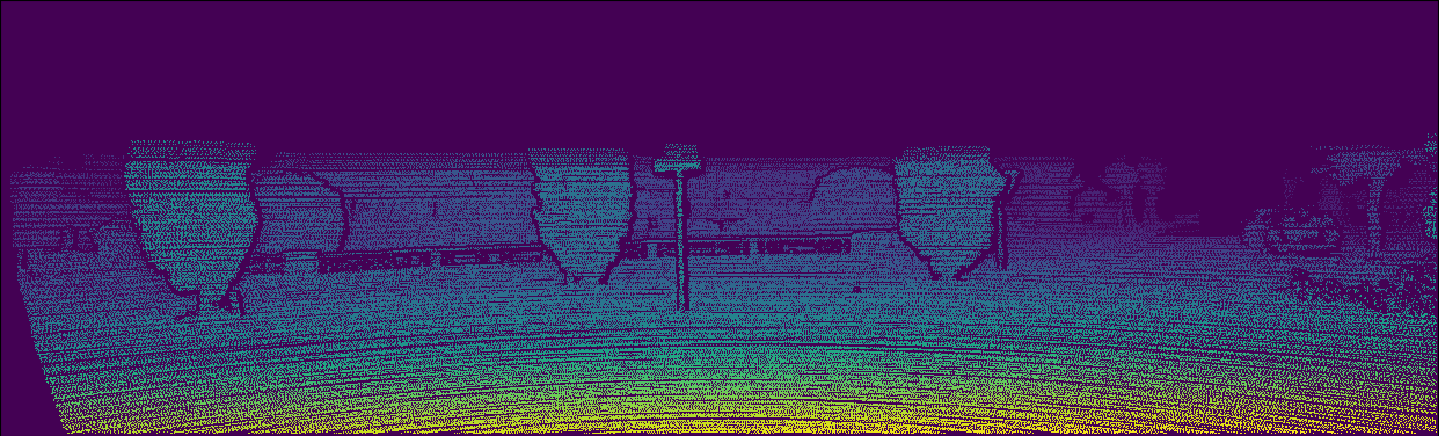
\includegraphics[width=\textwidth]{im4_disp_gt.png}
	\end{subfigure}

	\begin{subfigure}{0.45\textwidth}
		\caption{\e $\mathbf{window = 9 px}$ \g}
		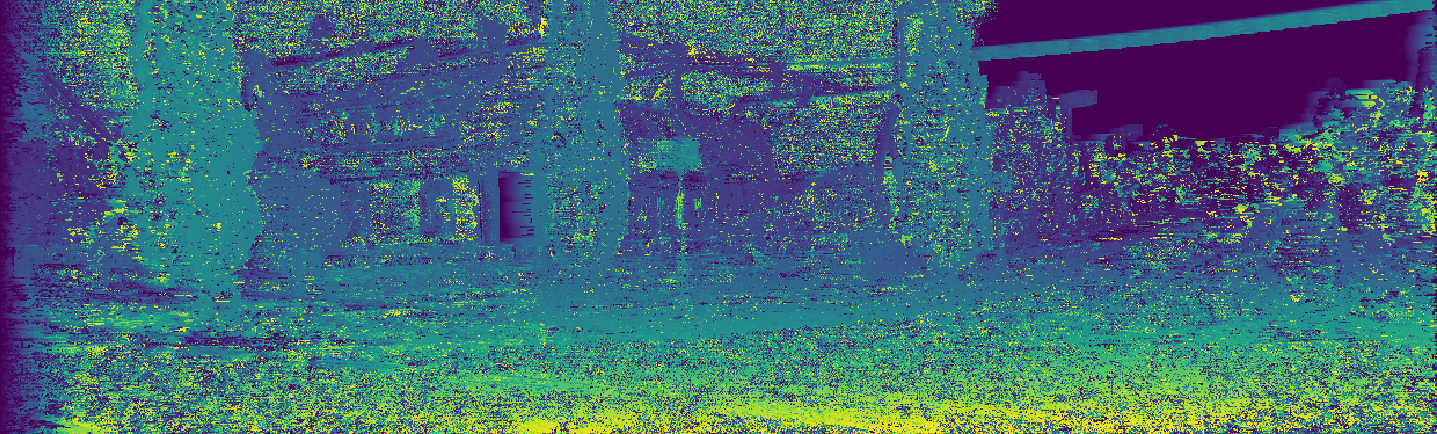
\includegraphics[width=\textwidth]{census_win_9.png}
	\end{subfigure}
	
	\begin{subfigure}{0.45\textwidth}
		\caption{\e $\mathbf{window = 15 px}$ \g}
		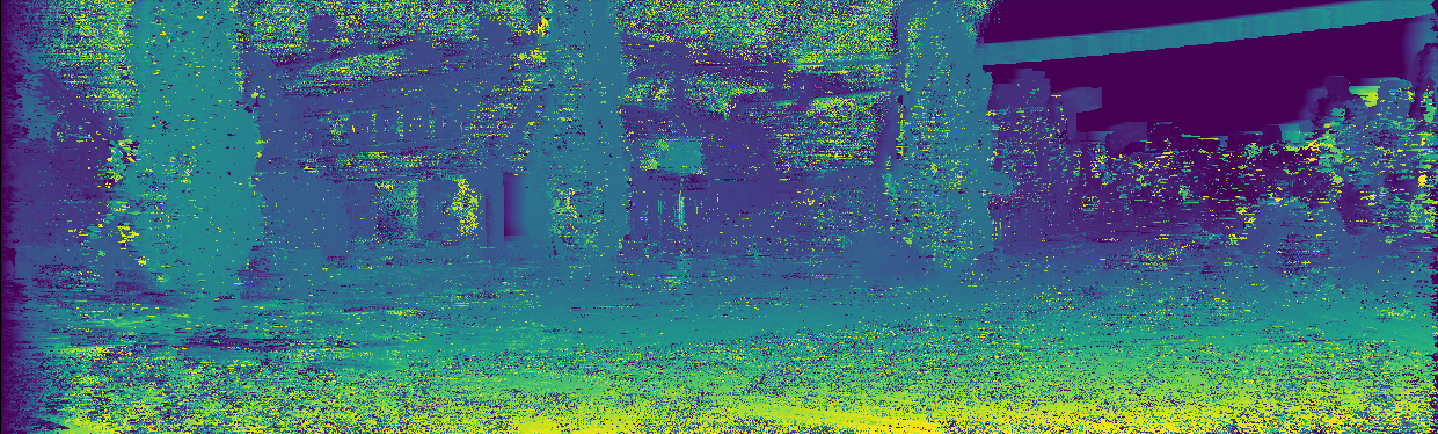
\includegraphics[width=\textwidth]{census_win_15.png}
	\end{subfigure}
	
	\begin{subfigure}{0.45\textwidth}
		\caption{\e $\mathbf{window = 21 px}$ \g}
		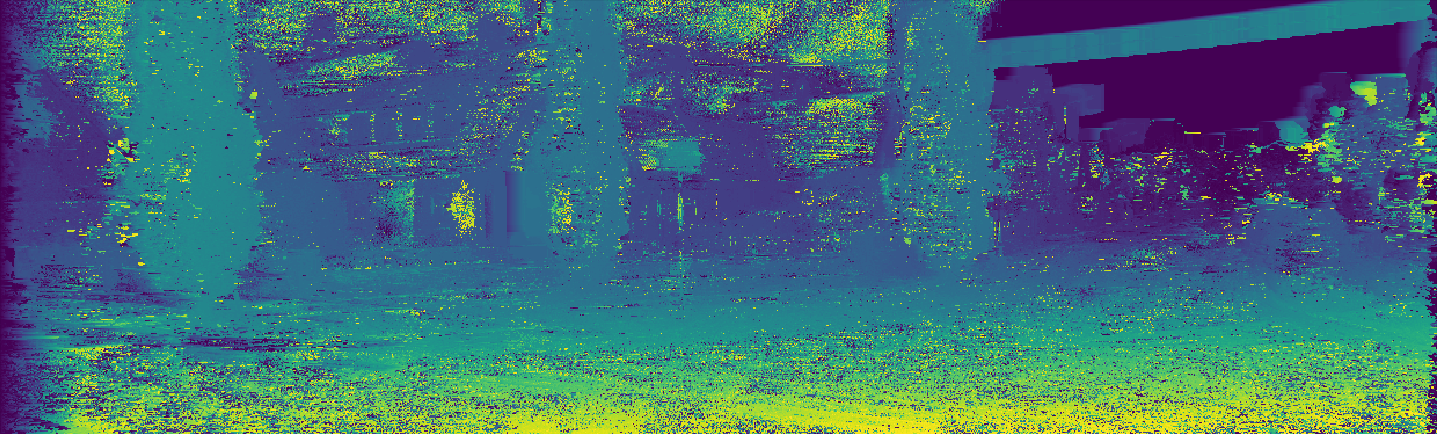
\includegraphics[width=\textwidth]{census_win_21.png}
	\end{subfigure}
	
	\begin{subfigure}{0.45\textwidth}
		\caption{\e $\mathbf{window = 27 px}$ \g}
		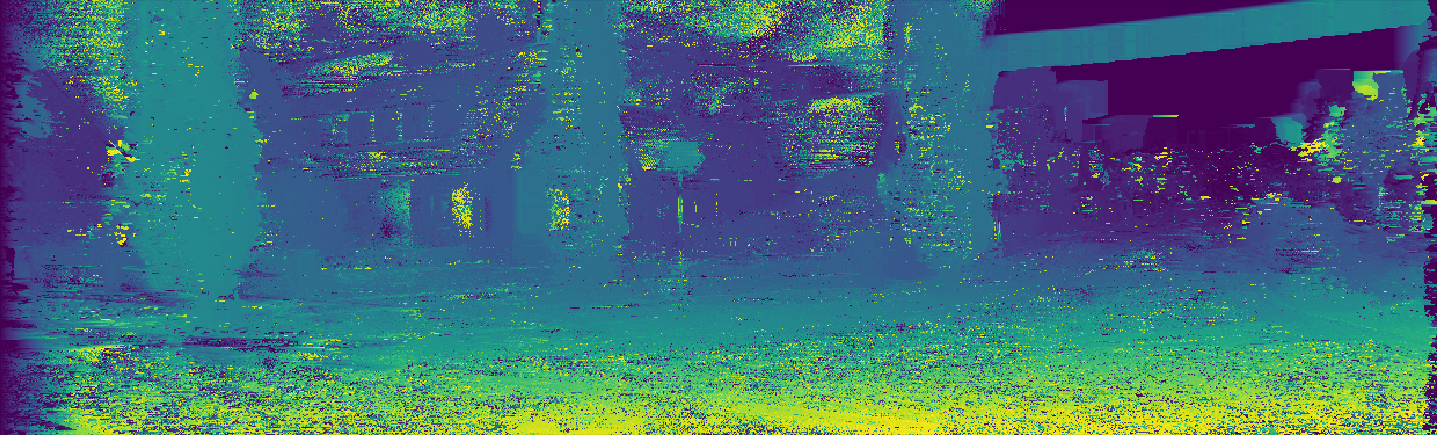
\includegraphics[width=\textwidth]{census_win_27.png}
	\end{subfigure}
	\begin{subfigure}{0.45\textwidth}
		\caption{\e Error: $32.27\%$ \g}
		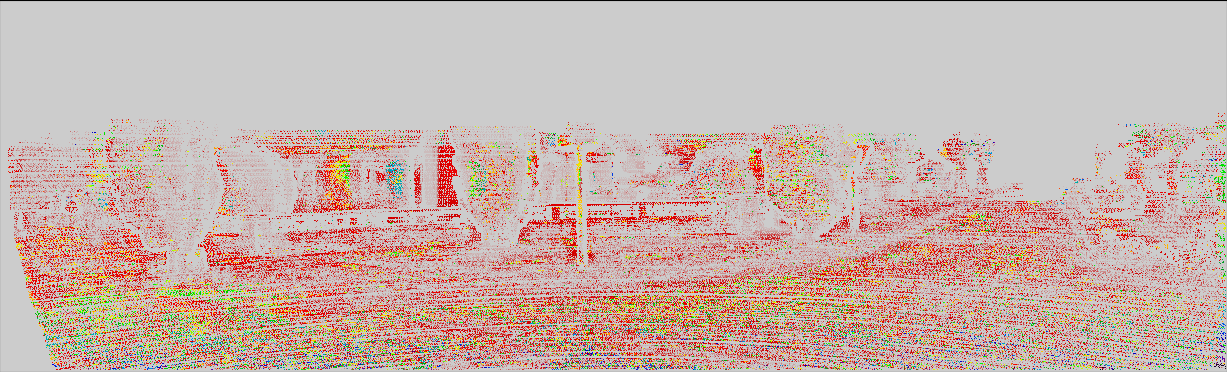
\includegraphics[width=\textwidth]{census_win_27_err.png}
	\end{subfigure}
	
	\begin{subfigure}{0.45\textwidth}
		\caption{\e $\mathbf{window = 33 px}$ \g}
		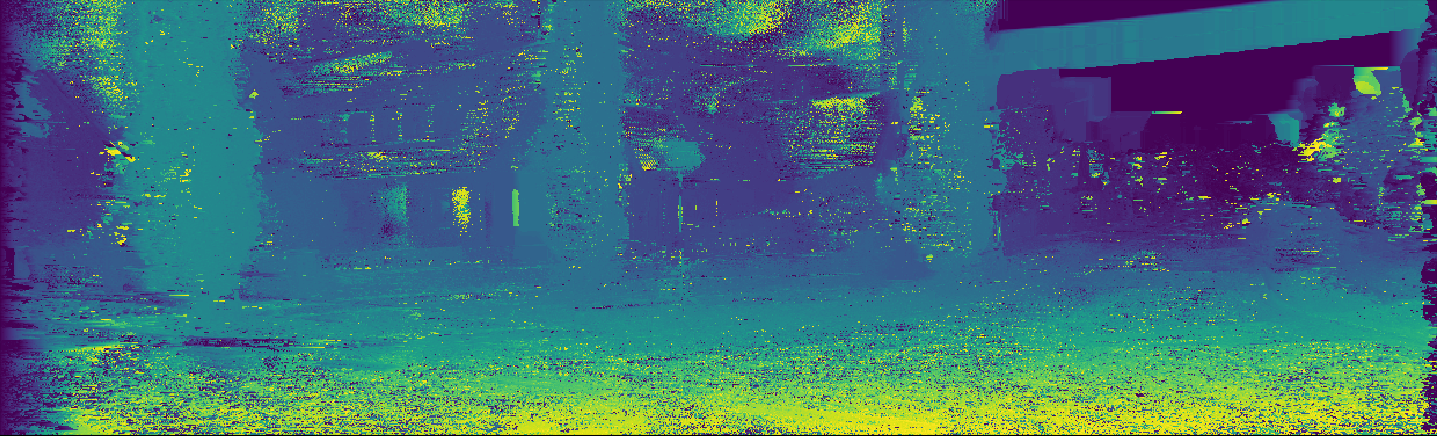
\includegraphics[width=\textwidth]{census_win_33.png}
	\end{subfigure}
	
	\begin{subfigure}{0.45\textwidth}
		\caption{\e $\mathbf{window = 39 px}$ \g}
		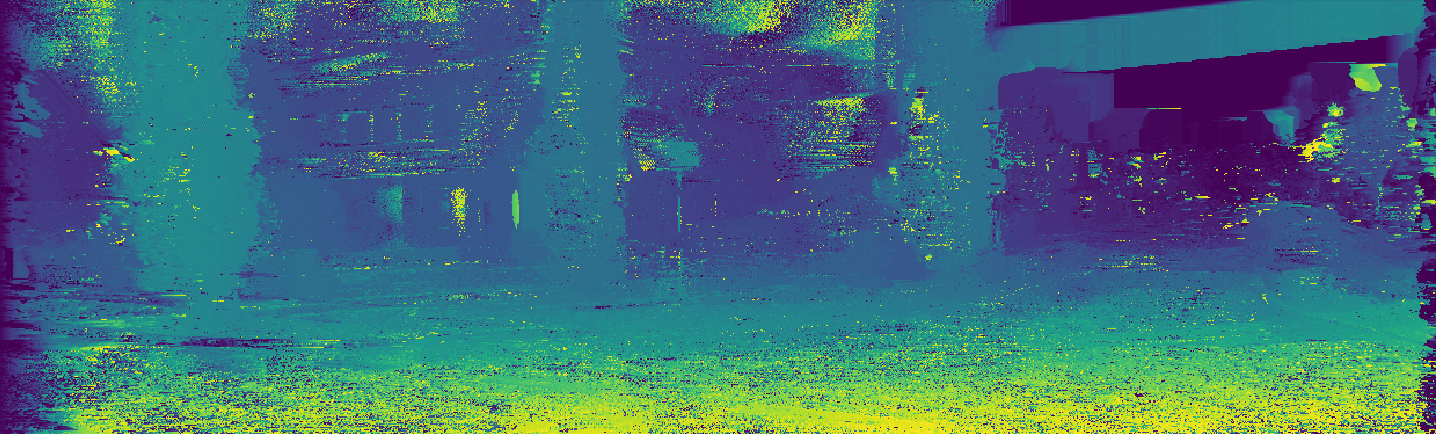
\includegraphics[width=\textwidth]{census_win_39.png}
	\end{subfigure}
	
	\caption{Μετασχηματισμός \e Census \g σε παράθυρα διαφορετικού μεγέθους.}
	\label{fig:census_multiple_windows}
\end{figure}


\subsubsection{Μέθοδος \texorpdfstring{\e AD-Census\g}{TEXT}}

Ο συνδυασμός του "αθροίσματος απόλυτων διαφορών" και μετασχηματισμού \e Census \g δημιουργεί την μέθοδο \e AD-Census. \g \citep{mei2011building}. Στο σχήμα \ref{fig:AD_Census_multiple_windows} φαίνεται ο χάρτης παράλλαξης για διαφορετικές τιμές παραθύρου. Οι υπολογισμοί έγιναν με τιμές παραμέτρων $\mathtt{l\_AD} = 10$, $\mathtt{l\_Census} = 30$. Βέλτιστη επίδοση πετυχαίνεται για επιλογή παραθύρου μεγέθους $\mathtt{window\_size} = 21\:px$ με ποσοστό απόλυτου σφάλματος $19.84\%$.

\begin{figure}
	\centering
	\begin{subfigure}{0.32\textwidth}
		\caption{$I^L$}
		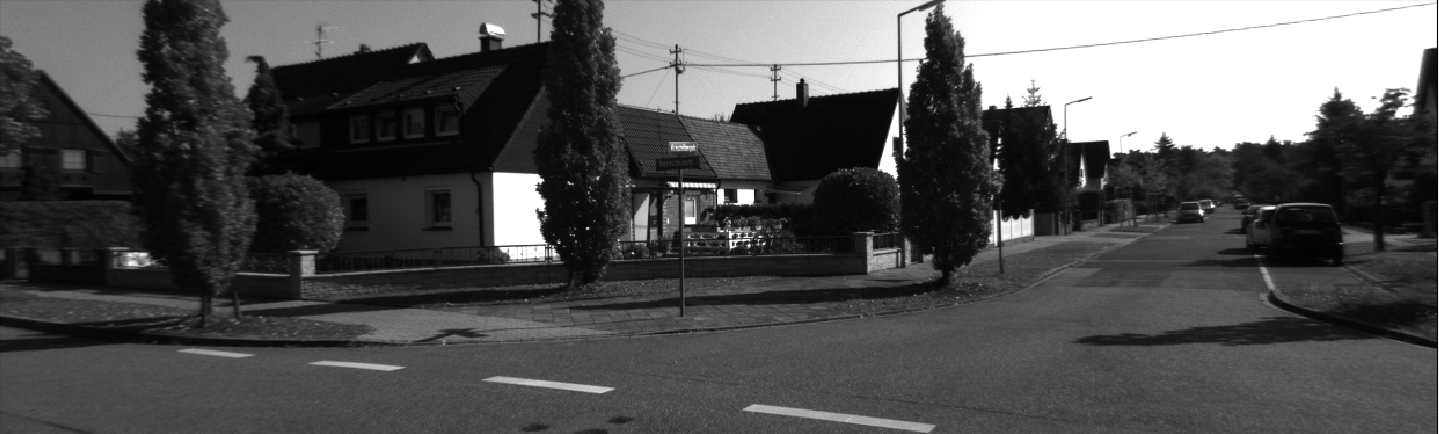
\includegraphics[width=\textwidth]{im4_imL.png}
	\end{subfigure}
	\begin{subfigure}{0.32\textwidth}
		\caption{$I^R$}
		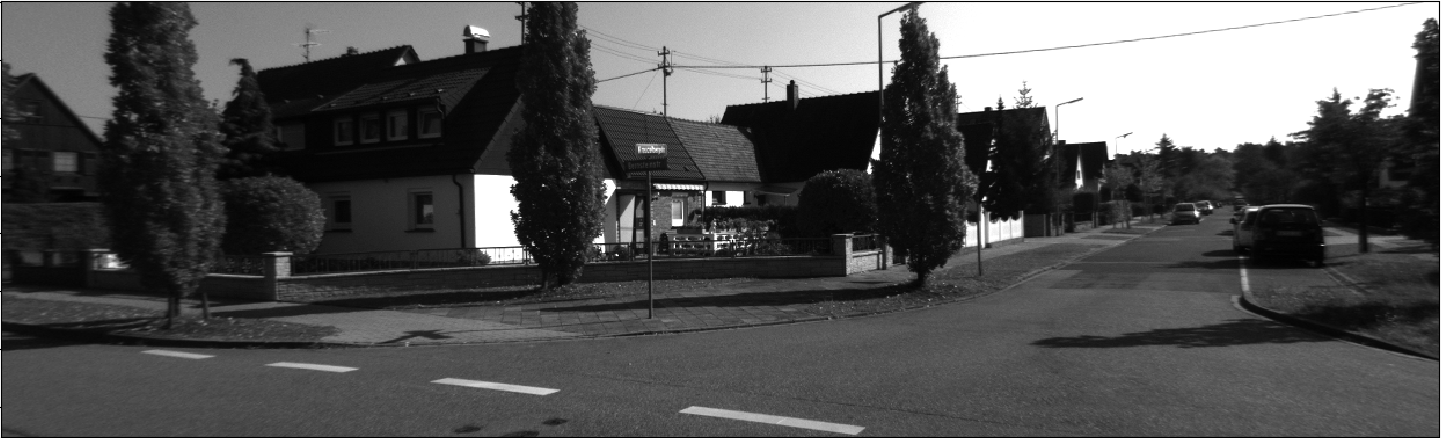
\includegraphics[width=\textwidth]{im4_imR.png}
	\end{subfigure}
	\begin{subfigure}{0.32\textwidth}
		\caption{\e $\mathbf{ground\_trouth}$ \g}
		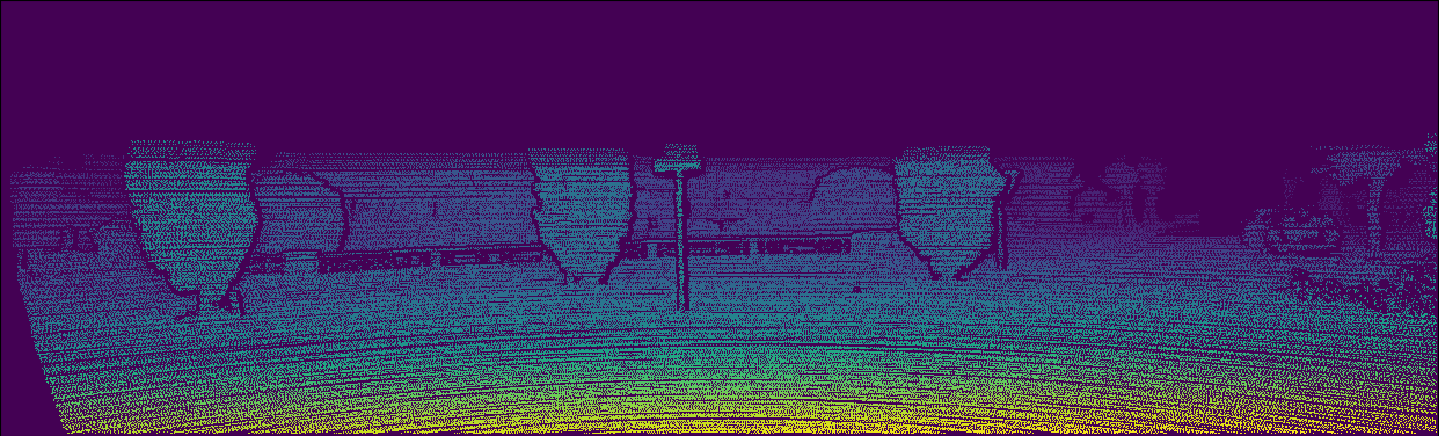
\includegraphics[width=\textwidth]{im4_disp_gt.png}
	\end{subfigure}

	\begin{subfigure}{0.45\textwidth}
		\caption{\e $\mathbf{window = 9 px}$ \g}
		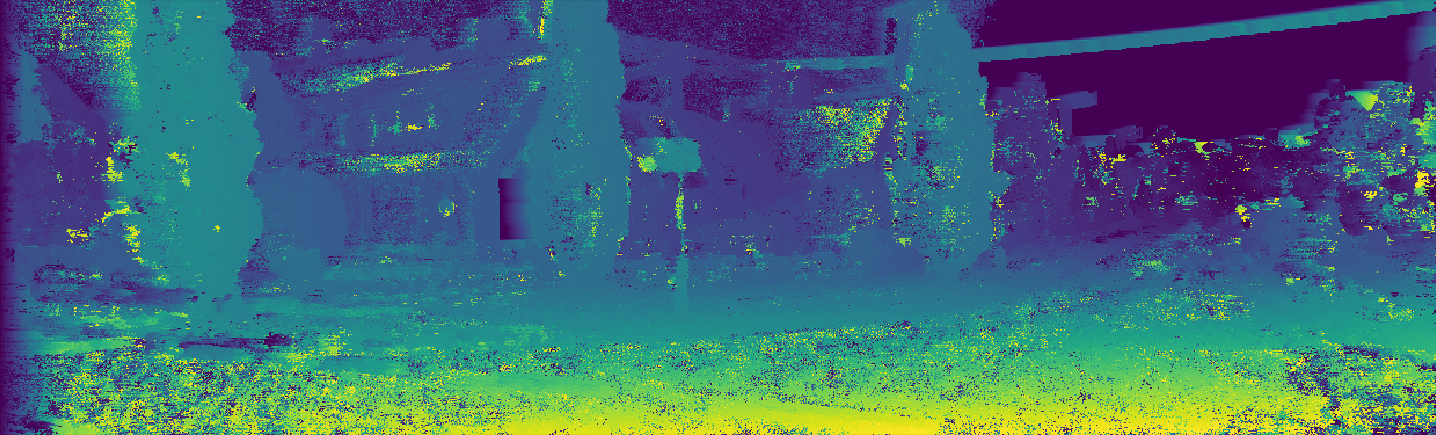
\includegraphics[width=\textwidth]{AD_Census_win_9.png}
	\end{subfigure}
	
	\begin{subfigure}{0.45\textwidth}
		\caption{\e $\mathbf{window = 15 px}$ \g}
		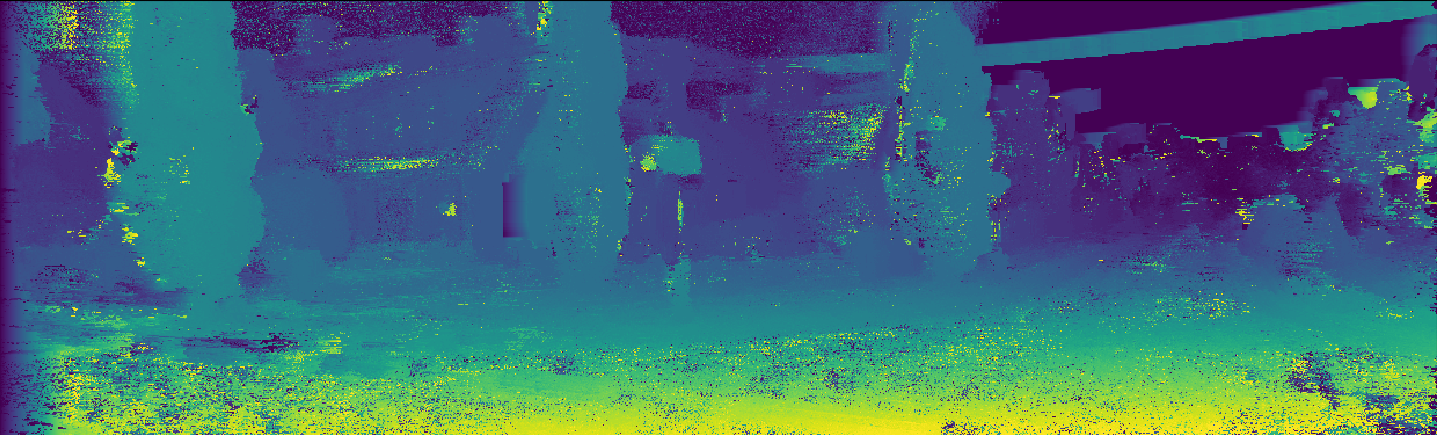
\includegraphics[width=\textwidth]{AD_Census_win_15.png}
	\end{subfigure}
	
	\begin{subfigure}{0.45\textwidth}
		\caption{\e $\mathbf{window = 21 px}$ \g}
		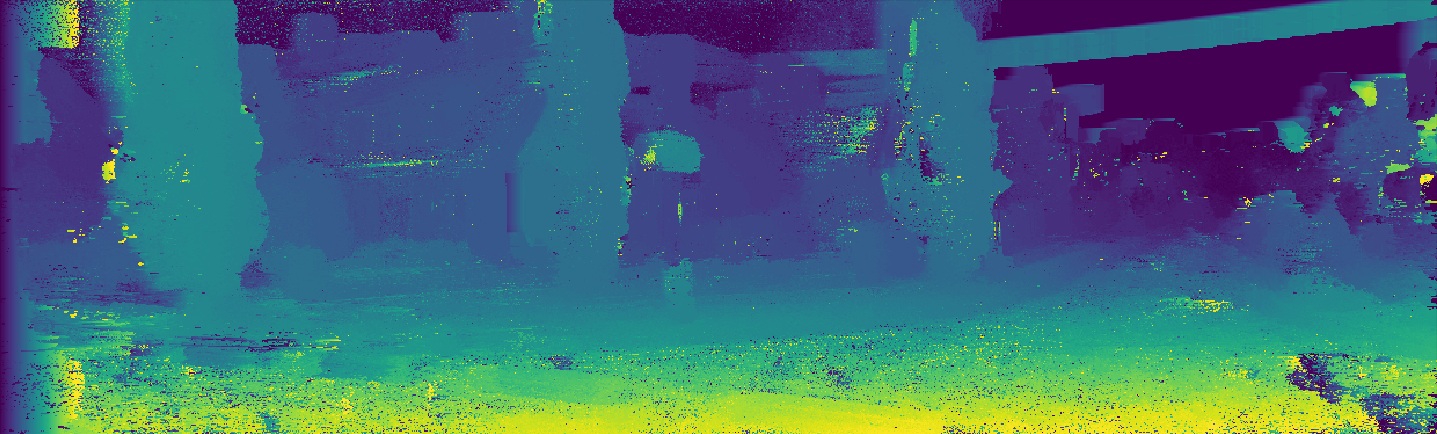
\includegraphics[width=\textwidth]{AD_Census_win_21.png}
	\end{subfigure}
	\begin{subfigure}{0.45\textwidth}
		\caption{\e Error: $19.84\%$ \g}
		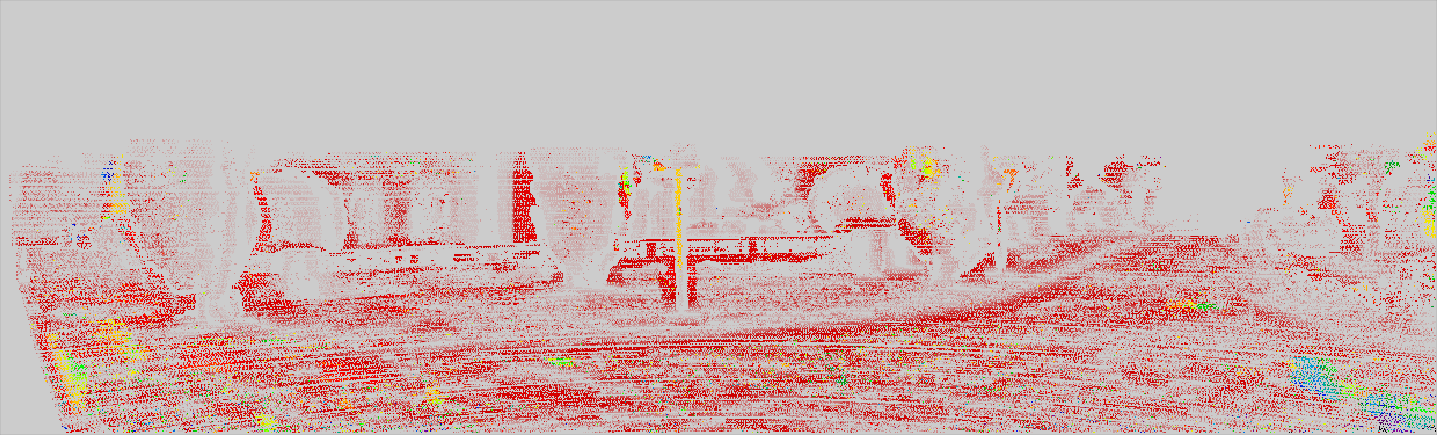
\includegraphics[width=\textwidth]{AD_Census_win_27_err.png}
	\end{subfigure}
	
	\begin{subfigure}{0.45\textwidth}
		\caption{\e $\mathbf{window = 27 px}$ \g}
		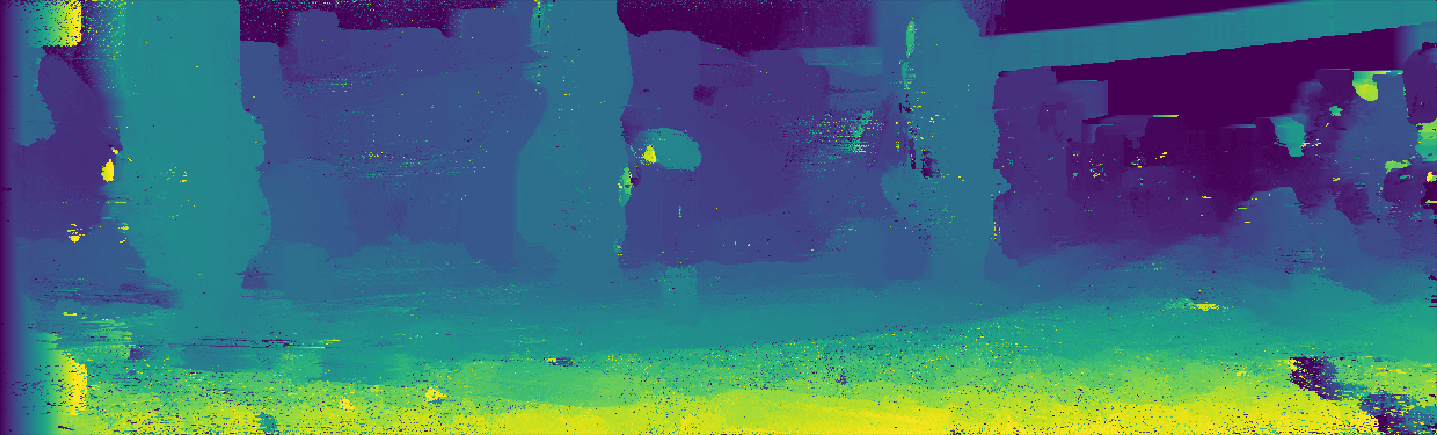
\includegraphics[width=\textwidth]{AD_Census_win_27.png}
	\end{subfigure}
	
	\begin{subfigure}{0.45\textwidth}
		\caption{\e $\mathbf{window = 33 px}$ \g}
		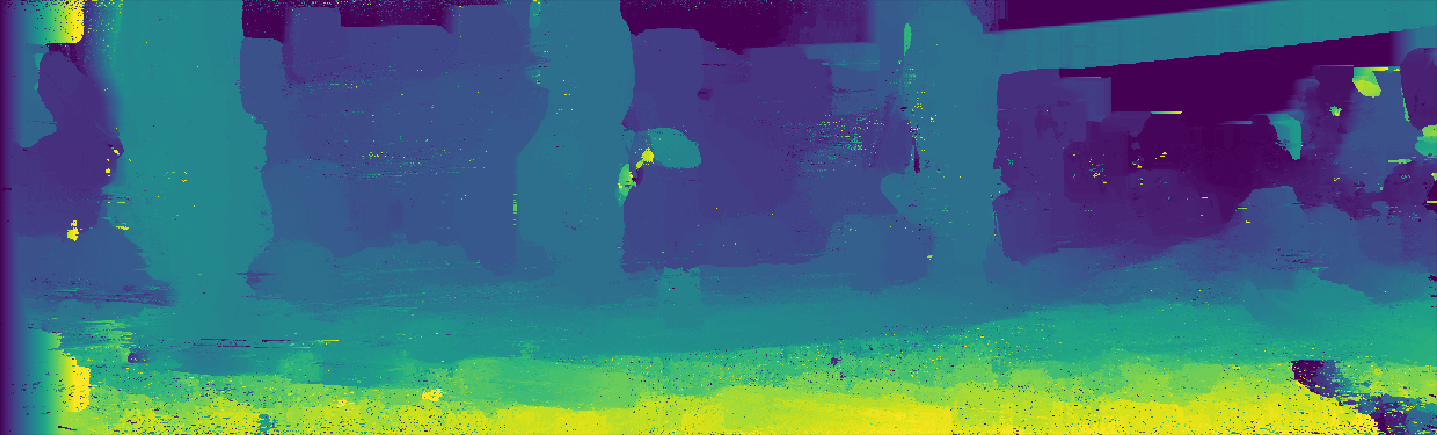
\includegraphics[width=\textwidth]{AD_Census_win_33.png}
	\end{subfigure}
	
	\begin{subfigure}{0.45\textwidth}
		\caption{\e $\mathbf{window = 39 px}$ \g}
		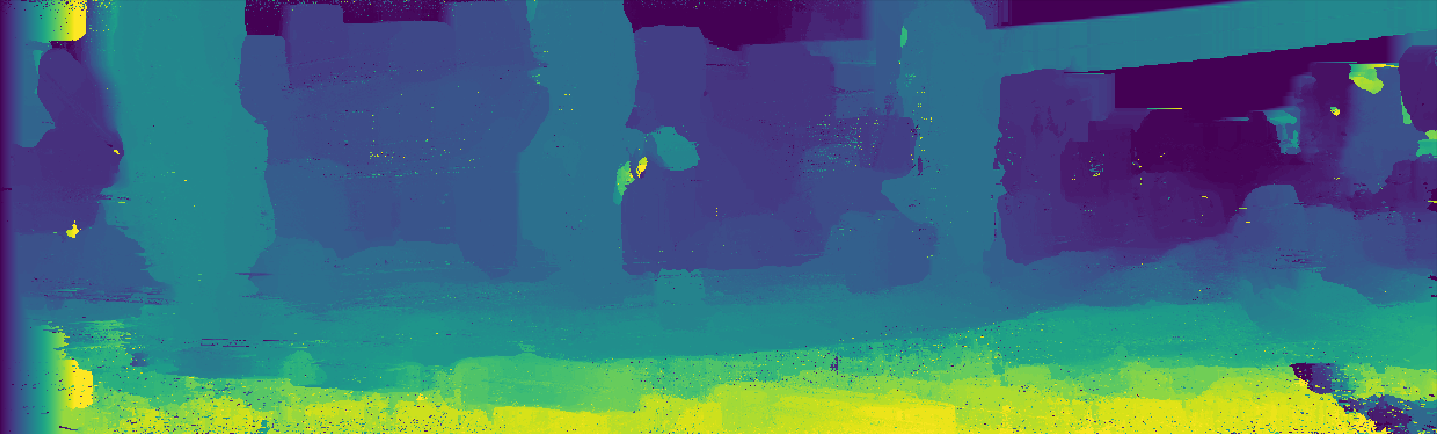
\includegraphics[width=\textwidth]{AD_Census_win_39.png}
	\end{subfigure}
	
	\caption{Μετασχηματισμός \e AD-Census \g σε παράθυρα διαφορετικού μεγέθους.}
	\label{fig:AD_Census_multiple_windows}
\end{figure}


\subsubsection{Σύγκριση μεθόδων}

Τα ποσοστά σφάλματος και τα απόλυτα σφάλματα των τριών παραπάνω μεθόδων για διαφορές τιμές παραθύρων άθροισης φαίνονται στα γραφήματα του σχήματος \ref{fig:all_handcrafted_methods}. Οι μετρήσεις δεν είναι αρκετά ευσταθείς καθώς έγιναν σε ένα μόνο στερεοσκοπικό ζεύγος εικόνων. \g Η μέθοδος \e AD-Census \g αν και εμφανίζει το δεύτερο καλύτερο αποτέλεσμα μετά την μέθοδο "αθροίσματος απόλυτων διαφορών" είναι η πιο αξιόπιστη σε συνδυασμό με τα βήματα της στερεοσκοπικής μεθόδου, γι' αυτό την επιλέγουμε για την σύγκριση με τα αποτελέσματα του νευρωνικού δικτύου.

\begin{figure}
	\centering	
	\begin{subfigure}{\textwidth}
		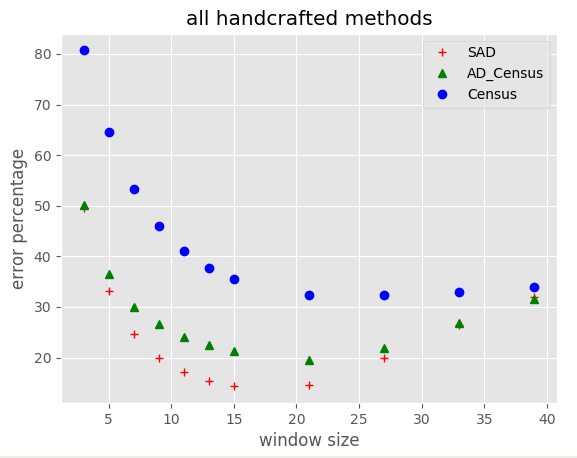
\includegraphics[width=\textwidth]{handcrafted_methods_errors.png}
		\caption{Μέσο απόλυτο σφάλμα με κατώφλι, για διαφορετικά μεγέθη παραθύρου.}
	\end{subfigure}
	
	\begin{subfigure}{\textwidth}
		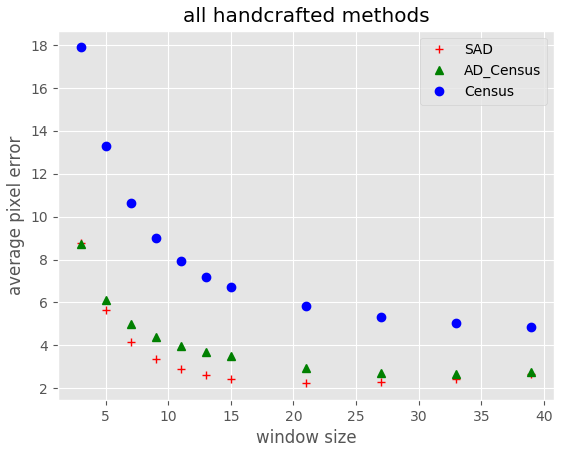
\includegraphics[width=\textwidth]{handcrafted_methods_mean_errors.png}
		\caption{Μέσο απόλυτο σφάλμα, για διαφορετικά μεγέθη παραθύρου.}
	\end{subfigure}
	\caption{Σύγκριση αποτελεσμάτων συμβατικών μεθόδων}
	\label{fig:all_handcrafted_methods}
\end{figure}


%%%%%%%%%%%%%%%%%%%%%%%%%%%%%%%%%%%%%%%%%%%%%%%%%%%%%%%%%%%%%%%%%%%%%%%%%%%%%%%%%%%%%%%%%%%%%%%%%%
%%%%%%%%%%%%%%%%%%%%%%%%%%%%%%%%%%%%%%%%%%%%%%%%%%%%%%%%%%%%%%%%%%%%%%%%%%%%%%%%%%%%%%%%%%%%%%%%%%
%%%%%%%%%%%%%%%%%%%%%%%%%%%%%%%%%%%%%%%%%%%%%%%%%%%%%%%%%%%%%%%%%%%%%%%%%%%%%%%%%%%%%%%%%%%%%%%%%%
\subsection{Νευρωνικό δίκτυο ταξινόμησης πολλαπλών κατηγοριών}

Για να μειώσουμε την υπολογιστική πολυπλοκότητα επιλέγουμε να προωθήσουμε ολόκληρες τις εικόνες $I^L, I^R$ του στερεοσκοπικού ζεύγους στους δύο κλάδους του σιαμαίου δικτύου, αντί να προωθούμε κάθε χωρίο τους ξεχωριστά. Στην έξοδό του παίρνουμε τους αντίστοιχους συνολικούς περιγραφείς της εικόνας:

$$I_{desc}^L = f_{siamese}(I^L), \quad I_{desc}^R = f_{siamese}(I^R), \: \text{όπου:} \: I_{desc}^L, I_{desc}^R \in \mathbb{R}^{m \times n \times F}  $$

Το κόστος ομοιότητας υπολογίζεται ως το αντίθετο του εσωτερικού γινομένου των τοπικών περιγραφέων των υπό σύγκριση χωρίων. Για λόγους ταχύτητας, υπολογίζουμε κάθε επίπεδο $d$ του πίνακα κόστους $C$ σε μια πράξη εσωτερικού γινομένου:

\e
\begin{lstlisting}[mathescape=true]
	for d in range(max_disparity + 1):
		C_d = $=-\mathbf{dot\_product}_{\mathbf{F}}(I_{desc}^L[:,d:,:],I_{desc}^R[:,:-d,:])$
		C[d,:,:] = C_d
\end{lstlisting}
\g

Στον πίνακα \ref{tbl:model} φαίνονται συμπυκνωμένα οι παραπάνω πράξεις με τους αντίστοιχους χρόνους που χρειάζονται για την εκτέλεσή τους. Στο γράφημα \ref{fig:cnn_time} φαίνονται οι χρόνοι εκτέλεσης για διαφορετικά μεγέθη εικόνων και μέγιστες παραλλάξεις.

Το δίκτυο είναι εκπαιδευμένο σε \e $\mathtt{patch\_size} = 19$. \g 

Στις εικόνες \ref{fig:im4_cnn} φαίνεται ο χάρτης παράλλαξης που προέκυψε από τον πίνακα κόστους που αρχικοποίησε το νευρωνικό δίκτυο. Το νευρωνικό δίκτυο έχει εκπαιδευτεί να συγκρίνει γειτονιές μεγέθους $\mathtt{patch\_size} = 19 \: px$. Το ποσοστό σφάλματος είναι $5.846\%$ και το μέσο απόλυτο σφάλμα $1.132\:px$. Η βελτίωση σε σχέση με τις προηγούμενες μεθόδους είναι έντονη και γενικεύεται στο σύνολο των σετ δεδομένων. 

\begin{table}[t]
\e
\centering
\resizebox{\linewidth}{!}{
\begin{tabular}{l|l|c|c}
& \g Περιγραφή Επιπέδων & \g Διαστάσεις & \g Χρόνος \e \\ \hline \hline
%
\multicolumn{3}{c}{\textbf{Local descriptors extraction \g(Εξαγωγή περιγραφέων)\e}} \\ \hline
\multicolumn{3}{c}{\textbf{Siamese network \g(Σιαμαίο δίκτυο)\e}} \\ \hline
& \g Eίσοδος \e $I^L, I^R$ &  H$\times$W$\times$1 & \\ \hline
1 & 3$\times$3 conv2d+BN+ReLU, F=64 & H$\times$W$\times$F & 0.06 sec\\
2 & 3$\times$3 conv2d+BN+ReLU, F=64 & H$\times$W$\times$F & 0.06 sec\\
\vdots &  \qquad \qquad  \vdots  & \vdots & \vdots		         \\
8 & 3$\times$3 conv2d+BN+ReLU, F=64 & H$\times$W$\times$F & 0.06 sec\\
9 & 3$\times$3 conv2d+BN (not ReLU), F=64 & H$\times$W$\times$F & 0.06 sec\\ \hline
& \g Έξοδος \e $I_{desc}^L,I_{desc}^R$ &  H$\times$W$\times$F \\ \hline \hline
%
\multicolumn{3}{c}{\textbf{\g Υπολογισμός κόστους ομοιότητας $\mathbf{C}_{\mathbf{d}}$ \e}} \\ \hline
10 & $\mathbf{C}_{\mathbf{d}}=-\mathbf{dot\_product}_{\mathbf{F}}(I_{desc}^L[:,d:,:],I_{desc}^R[:,:-d,:])$ & 1$\times$H$\times$W & 0.95 sec
\end{tabular}}
	\caption{\g Περίληψη επιπέδων δικτύου ταξινόμησης πολλαπλών επιπέδων. Όλα τα βήματα υπολογίζονται μια φορά, εκτός του βήματος 10 που υπολογίζεται ξεχωριστά για κάθε διαφορετικό επίπεδο $d$. Οι χρόνοι έχουν υπολογιστεί για μία μέση φωτογραφία με \e $H=400,W=1200, \mathtt{max\_disparity}=150$. \g}
	\label{tbl:model}
\g
\end{table}

\begin{figure}
	\centering
	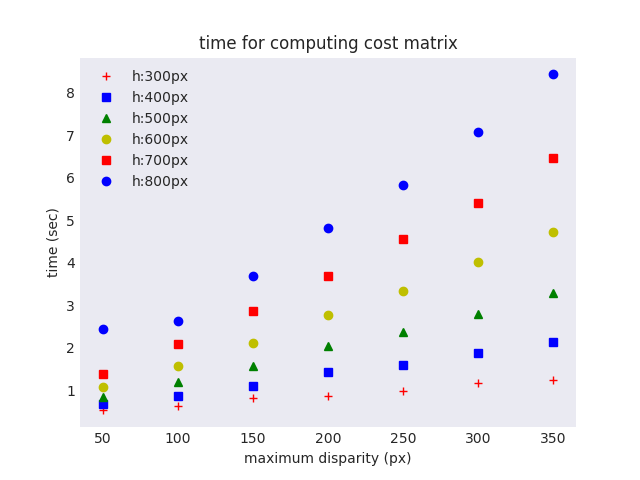
\includegraphics[width=\textwidth]{luo19_times.png}
	\caption{Χρόνος υπολογισμού του πίνακα κόστους από το νευρωνικό δίκτυο συναρτήσει του μεγέθους της εικόνας και της μέγιστης παράλλαξης. Το μέγεθος της εικόνας εισόδου είναι $h\times\dfrac{16}{9}h \: px$. Παρατηρούμε ότι οι χρόνοι δεν ξεπερνούν τα $9\:sec$ ακόμη και για εικόνα $800\times 1420$ (μεγαλύτερη ανάλυση από το όριο του \e high-definition) \g και μέγιστη παράλλαξη τα $350\:px$. Για εικόνες μεγαλύτερου γινομένου $h\times\dfrac{16}{9}h \times \mathtt{max\_disparity}$ δεν επαρκούσε η μνήμη της κάρτας γραφικών.}
	\label{fig:cnn_time}
\end{figure}

\begin{figure}
	\centering
	\begin{subfigure}{0.32\textwidth}
		\caption{$I^L$}
		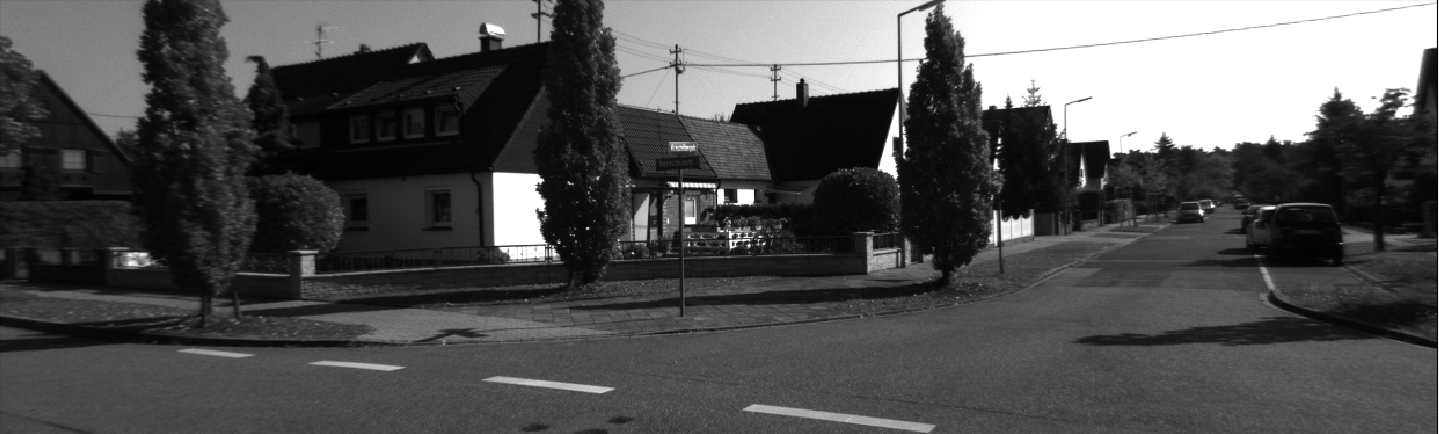
\includegraphics[width=\textwidth]{im4_imL.png}
	\end{subfigure}
	\begin{subfigure}{0.32\textwidth}
		\caption{$I^R$}
		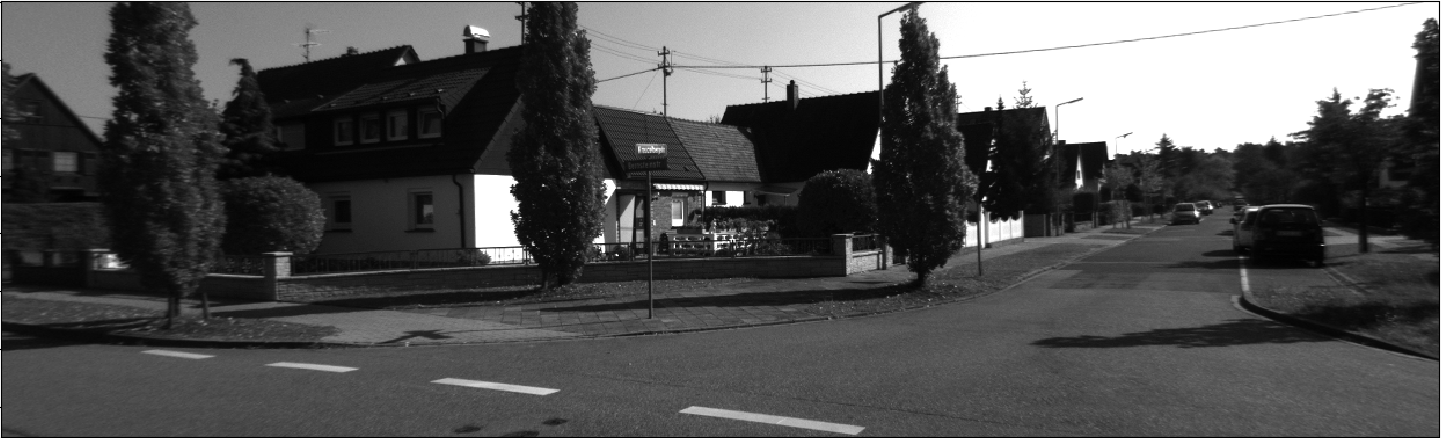
\includegraphics[width=\textwidth]{im4_imR.png}
	\end{subfigure}
	\begin{subfigure}{0.32\textwidth}
		\caption{\e $\mathbf{ground\_trouth}$ \g}
		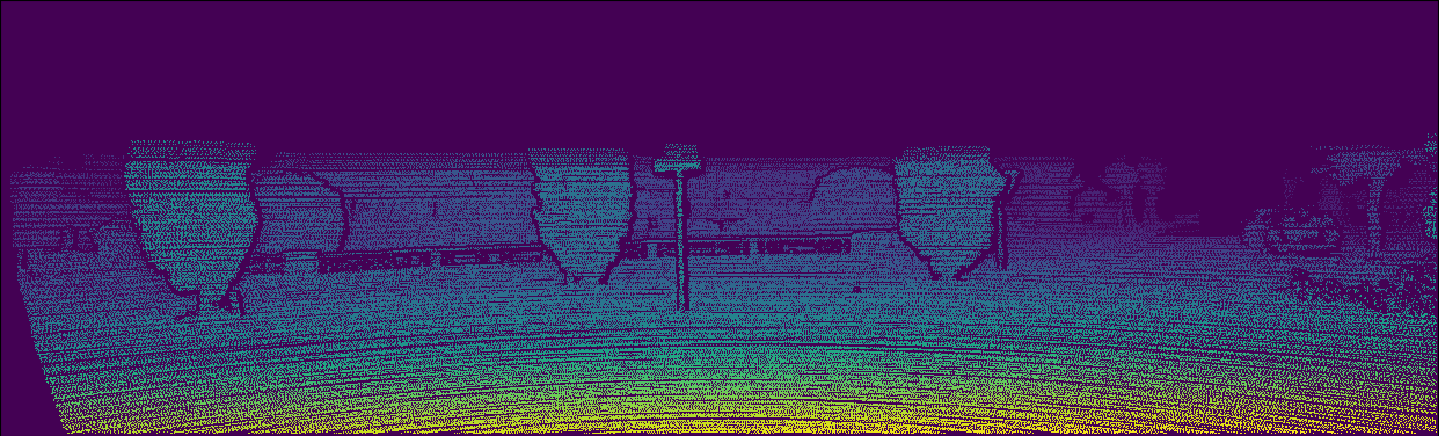
\includegraphics[width=\textwidth]{im4_disp_gt.png}
	\end{subfigure}

	\begin{subfigure}{0.8\textwidth}
		\caption{Χάρτης παράλλαξης νευρωνικού δικτύου}
		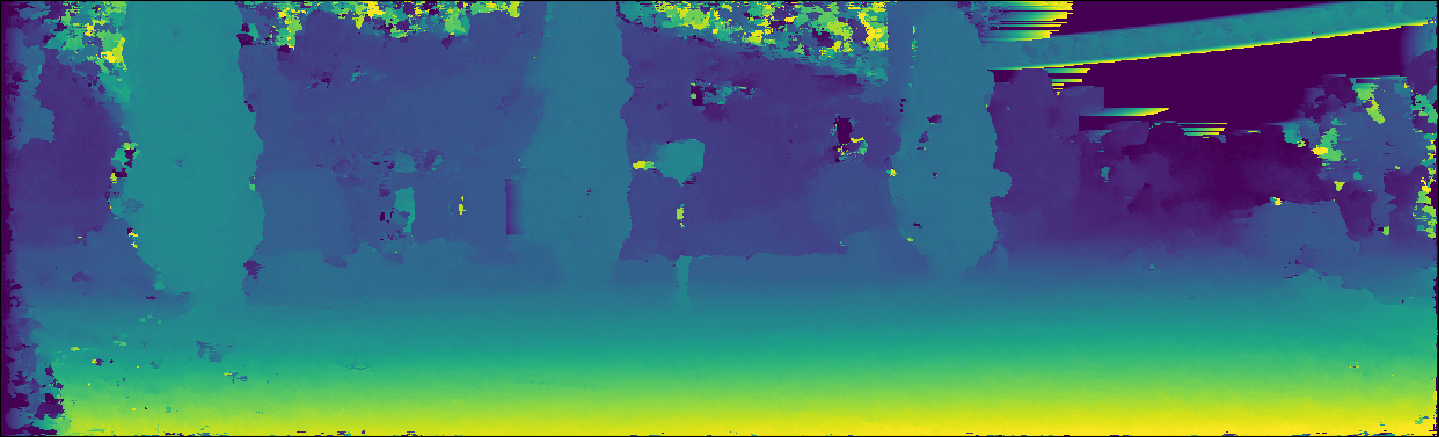
\includegraphics[width=\textwidth]{im4_luo_cnn_disp.png}
	\end{subfigure}
	
	\begin{subfigure}{0.8\textwidth}
		\caption{\e average pixel error: $1.132$ px \g}
		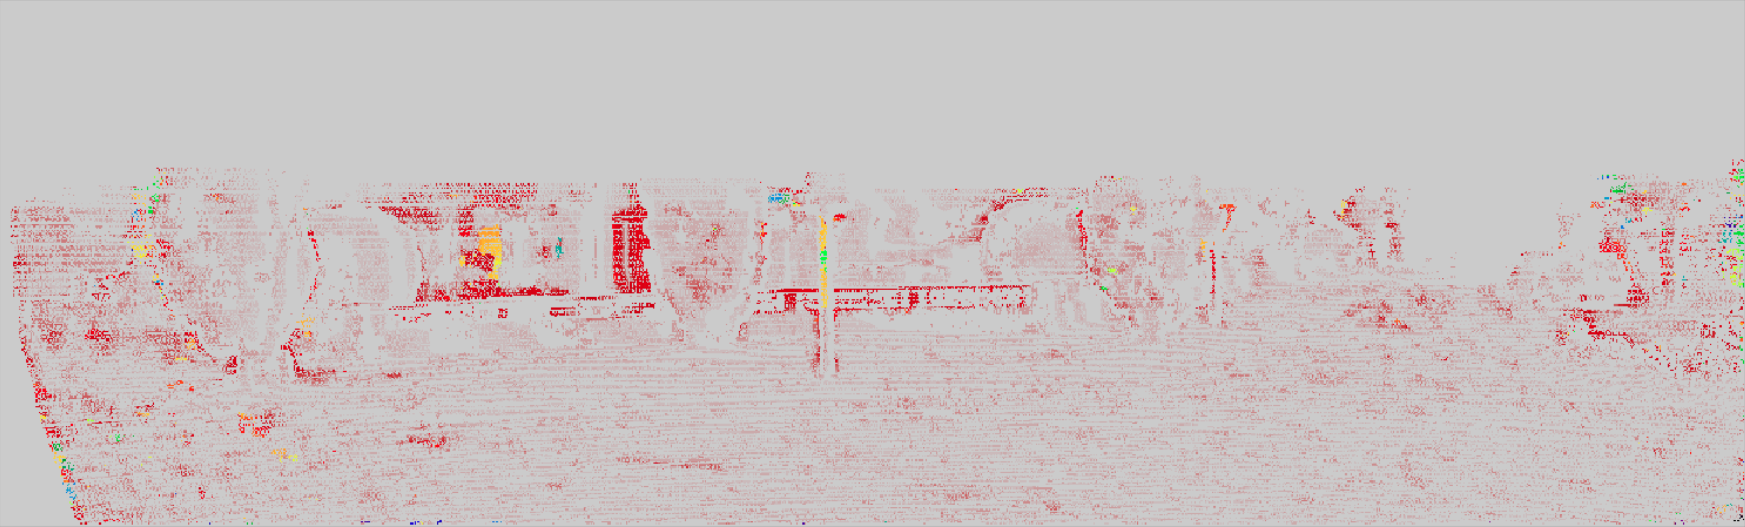
\includegraphics[width=\textwidth]{im4_luo_cnn_err_im.png}
		
\includegraphics[width=\textwidth]{error_colorbar.png}
	\end{subfigure}
	
	\begin{subfigure}{0.8\textwidth}
		\caption{\e Error: $5.846\%$ \g}
		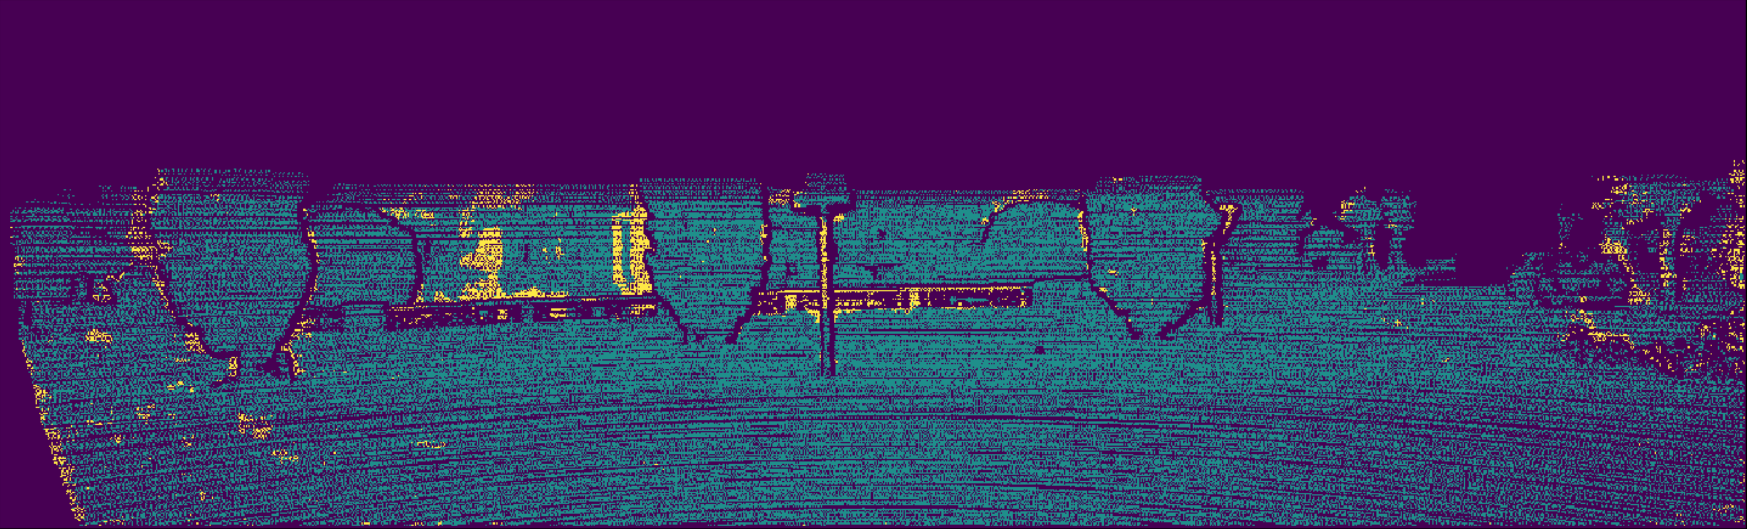
\includegraphics[width=\textwidth]{im4_luo_cnn_err_im_thres.png}
	\end{subfigure}
	
	\caption{Χάρτης παράλλαξης υπολογισμένος με βάση τον πίνακα κόστους που αρχικοποιεί το νευρωνικό δίκτυο.}
	\label{fig:im4_cnn}
\end{figure}


%%%%%%%%%%%%%%%%%%%%%%%%%%%%%%%%%%%%%%%%%%%%%%%%%%%%%%%%%%%%%%%%%%%%%%%%%%%%%%%%%%%%%%%%%%%%%%%%%%%%%%%%%%%%%%%
%%%%%%%%%%%%%%%%%%%%%%%%%%%%%%%%%%%%%%%%%%%%%%%%%%%%%%%%%%%%%%%%%%%%%%%%%%%%%%%%%%%%%%%%%%%%%%%%%%%%%%%%%%%%%%%
\section{Στερεοσκοπική Μέθοδος}

Η μελέτη των βημάτων γίνεται παρουσιάζοντας τα αποτελέσματα πριν και μετά από το κάθε βήμα της στερεοσκοπικής μεθόδου. Θα δοκιμάζονται οι πίνακες κόστους και οι χάρτες παράλλαξης που έχουν προκύψει από την μέθοδο \e AD-Census \g και το νευρωνικό δίκτυο.

\subsection{Άθροιση κόστους σε προσαρμόσιμη περιοχή υποστήριξης}

Οι υπολογισμοί υλοποιούνται με τιμές παραμέτρων $\mathtt{intensity\_threshold = 0.13}$ και  $\mathtt{distance\_threshold = 5}$ που κάνουν τον αλγόριθμο αρκετά ευαίσθητο στην ανεύρεση ακμών και το εύρος των περιοχών υποστήριξης περιορισμένο. Έτσι έχουμε αρκετά εχέγγυα ότι δεν θα περάσουμε σχεδόν ποτέ από μια επιφάνεια σε μια άλλη, με κόστος οι περιοχές υποστήριξης να περιορίζονται σε πολύ μικρότερα εμβαδά απ' τη συνολική επιφάνεια του αντικειμένου πάνω στο οποίο υπολογίζονται. Αυτή η επιλογή "μικρού ρίσκου" δίνει τη δυνατότητα η επανάληψη του αλγορίθμου πολλές φορές να εξομαλύνει τον χάρτη παράλλαξης χωρίς να καταστρέφει (θολώνει) τις ακμές, όπως επιβεβαιώνεται και στα γραφήματα της εικόνας \ref{fig:cbca_results}. Οφείλουμε να σχολιάσουμε ότι τα βήματα της άθροισης κόστους σε προσαρμόσιμη περιοχή υποστήριξης και της ημι-καθολικής αντιστοίχησης έχουν όμοιο στόχο: την εξομάλυνση του χάρτη παράλλαξης. Επομένως η εξαντλητική χρησιμοποίηση του ενός εργαλείου, για παράδειγμα την εφαρμογή του παρόντος βήματος επαναληπτικά $\mathtt{cbca\_iter}>10$ φορές, μειώνει εξαιρετικά την επίδραση του έτερου. Παρατηρούμε ότι στην περίπτωση που τα κόστη έχουν αρχικοποιηθεί με νευρωνικό δίκτυο, η επαναληπτική χρήση της "άθροισης κόστους" βελτιώνει το αποτέλεσμα διαρκώς μέχρι και τις $40$ επαναλήψεις όπου το ποσοστό σφάλματος έχει πέσει στο $3.2\%$. Αντίθετα στην περίπτωση αρχικοποίησης με \e AD-Census \g η βελτίωση τελματώνει στις $25$ επαναλήψεις με ποσοστό σφάλματος $7.8\%$. Πρέπει να επισημάνουμε ότι τα αποτελέσματα της "άθροισης κόστους" δεν είναι πάντα το ίδιο ευεργετικά όσο το συγκεκριμένο παράδειγμα. Γενικότερα, συνηθίζεται η βελτίωση του σφάλματος, σε συνδυασμό με το επόμενο βήμα της ημικαθολικής αντιστοίχησης, να σταματάει μετά τις $3$ επαναλήψεις. Έτσι, συνήθως επιλέγουμε μια τιμή στο εύρος $[0,5]$.

\begin{figure}
	\centering
	\begin{subfigure}{0.48\textwidth}
		\includegraphics[width=\textwidth]{cnn_cbca_error.png}
	\end{subfigure}
	\begin{subfigure}{0.48\textwidth}
		\includegraphics[width=\textwidth]{cnn_cbca_mean_error.png}
	\end{subfigure}
	
	\begin{subfigure}{0.48\textwidth}
		\includegraphics[width=\textwidth]{AD_census_cbca_error.png}
	\end{subfigure}
	\begin{subfigure}{0.48\textwidth}
		\includegraphics[width=\textwidth]{AD_census_cbca_mean_error.png}
	\end{subfigure}
	
	\begin{subfigure}{0.48\textwidth}
		\includegraphics[width=\textwidth]{cnn_cbca_iter_0.png}
		\caption{\e cnn \g}
	\end{subfigure}
	\begin{subfigure}{0.48\textwidth}
		\includegraphics[width=\textwidth]{cnn_cbca_iter_2.png}
		\caption{\e cnn + cbca iter 2 \g}
	\end{subfigure}
	
	\begin{subfigure}{0.48\textwidth}
		\includegraphics[width=\textwidth]{AD_census_cbca_iter_0.png}
		\caption{\e AD-Census iter 0 \g}
	\end{subfigure}
	\begin{subfigure}{0.48\textwidth}
		\includegraphics[width=\textwidth]{AD_census_cbca_iter_2.png}
		\caption{\e AD-Census iter 2 \g}
	\end{subfigure}
	\caption{Τα αποτελέσματα της μεθόδου \e cross-based cost aggregation \g συναρτήσει των επαναλήψεων εφαρμογής της.}
	\label{fig:cbca_results}
\end{figure}

\subsection{Ημι-καθολική αντιστοίχηση}

Επιλέγουμε τιμές παραμέτρων:
\begin{itemize}
\item $\mathtt{P1\_ref} = 1.5$
\item $\mathtt{P1\_ref} = 30$
\item $\mathtt{thres} = 0.13$
\item $\mathtt{big\_factor} = 6$
\item $\mathtt{small\_factor} = 3$
\end{itemize}

Επιλέγουμε το ίδιο όριο στη διαφορά φωτεινότητας $\mathtt{thres}$ με την μέθοδο "άθροισης κόστους". Η μέθοδος \e AD-Census \g μαζί με την ημικαθολική αντιστοίχηση εμφανίζουν σφάλμα $5.993\%$, κατά δύο ποσοστιαίες μονάδες μικρότερο σε σχέση με τον συνδυασμό \e AD-Census \g και \e cbca. \g Το νευρωνικό δίκτυο μαζί με την ημικαθολική αντιστοίχηση εμφανίζει σφάλμα $4.324\%$. Με την παρεμβολή και της μεθόδου \e cbca \g για δύο επαναλήψεις το σφάλμα μειώνεται στο $4.054\%$, ενώ η βέλτιστη επίδοσή του εμφανίζεται με παρεμβολή της μεθόδου \e cbca \g για $30$ επαναλήψεις στο $2,97\%$.


\begin{figure}
	\centering
	\begin{subfigure}{0.32\textwidth}
		\caption{$I^L$}
		\includegraphics[width=\textwidth]{im4_imL.png}
	\end{subfigure}
	\begin{subfigure}{0.32\textwidth}
		\caption{$I^R$}
		\includegraphics[width=\textwidth]{im4_imR.png}
	\end{subfigure}
	\begin{subfigure}{0.32\textwidth}
		\caption{\e $\mathbf{ground\_trouth}$ \g}
		\includegraphics[width=\textwidth]{im4_disp_gt.png}
	\end{subfigure}

	\begin{subfigure}{0.32\textwidth}
		\caption{\e AD Census + sgm \g : χάρτης παράλλαξης}
		\includegraphics[width=\textwidth]{AD_Census_sgm.png}
	\end{subfigure}
	\begin{subfigure}{0.32\textwidth}
		\caption{\e AD Census + sgm : Error $0.925$ px}
		\includegraphics[width=\textwidth]{AD_Census_sgm_error.png}
	\end{subfigure}
	\begin{subfigure}{0.32\textwidth}
		\caption{\e AD Census + sgm : Error $5.993\%$}
		\includegraphics[width=\textwidth]{AD_Census_sgm_error_thres.png}
	\end{subfigure}
	
	\begin{subfigure}{0.32\textwidth}
		\caption{\e cnn + sgm \g : χάρτης παράλλαξης}
		\includegraphics[width=\textwidth]{cnn_sgm.png}
	\end{subfigure}
	\begin{subfigure}{0.32\textwidth}
		\caption{\e cnn + sgm : Error $0.893$ px}
		\includegraphics[width=\textwidth]{cnn_sgm_error.png}
	\end{subfigure}
	\begin{subfigure}{0.32\textwidth}
		\caption{\e cnn + sgm : Error $4.324\%$}
		\includegraphics[width=\textwidth]{cnn_sgm_error_thres.png}
	\end{subfigure}
	
	\begin{subfigure}{0.32\textwidth}
		\caption{\e cnn + cbca 2 + sgm \g : χάρτης παράλλαξης}
		\includegraphics[width=\textwidth]{cnn_cbca2_sgm.png}
	\end{subfigure}
	\begin{subfigure}{0.32\textwidth}
		\caption{\e cnn + cbca 2 + sgm : Error $0.82$ px}
		\includegraphics[width=\textwidth]{cnn_cbca2_sgm_error.png}
	\end{subfigure}
	\begin{subfigure}{0.32\textwidth}
		\caption{\e cnn + cbca 2 + sgm : Error $4.054\%$}
		\includegraphics[width=\textwidth]{cnn_cbca2_sgm_error_thres.png}
	\end{subfigure}
	
		\begin{subfigure}{0.32\textwidth}
		\caption{\e cnn + cbca 30 + sgm :\g χάρτης παράλλαξης}
		\includegraphics[width=\textwidth]{cnn_cbca30_sgm.png}
	\end{subfigure}
	\begin{subfigure}{0.32\textwidth}
		\caption{\e cnn + cbca 30 + sgm : Error $0.683$ px}
		\includegraphics[width=\textwidth]{cnn_cbca30_sgm_error.png}
	\end{subfigure}
	\begin{subfigure}{0.32\textwidth}
		\caption{\e cnn + cbca 30 + sgm : Error $2.97\%$}
		\includegraphics[width=\textwidth]{cnn_cbca30_sgm_error_thres.png}
	\end{subfigure}
	
	\caption{Παραδείγματα εφαρμογής \e semi global matching. \g}
	\label{fig:sgm}
\end{figure}

\subsection{Εντοπισμός εξωκείμενων τιμών στον χάρτη παράλλαξης}

Εφαρμόζουμε τον αλγόριθμο εντοπισμού εξωκείμενων τιμών στις μέχρι τώρα βέλτιστες επιδόσεις. Στον συνδυασμό \e AD-Census + sgm \g η εφαρμογή του αλγορίθμου βελτιώνει το σφάλμα κατά $0.55\%$ στο $5.44\%$, ενώ στον συνδυασμό \e AD-Census + cbca30 + sgm \g κατά $0.1\%$ στο $2.87\%$.

\begin{figure}
	\centering
	\begin{subfigure}{0.32\textwidth}
		\caption{$I^L$}
		\includegraphics[width=\textwidth]{im4_imL.png}
	\end{subfigure}
	\begin{subfigure}{0.32\textwidth}
		\caption{$I^R$}
		\includegraphics[width=\textwidth]{im4_imR.png}
	\end{subfigure}
	\begin{subfigure}{0.32\textwidth}
		\caption{\e $\mathbf{ground\_trouth}$ \g}
		\includegraphics[width=\textwidth]{im4_disp_gt.png}
	\end{subfigure}

	\begin{subfigure}{0.32\textwidth}
		\caption{\e AD Census + sgm + outliers\g : χάρτης παράλλαξης}
		\includegraphics[width=\textwidth]{AD_Census_sgm_outliers.png}
	\end{subfigure}
	\begin{subfigure}{0.32\textwidth}
		\caption{\e AD Census + sgm + outliers: Error $0.882$ px}
		\includegraphics[width=\textwidth]{AD_Census_sgm_outliers_error.png}
	\end{subfigure}
	\begin{subfigure}{0.32\textwidth}
		\caption{\e AD Census + sgm + outliers: Error $5.44\%$}
		\includegraphics[width=\textwidth]{AD_Census_sgm_outliers_error_thres.png}
	\end{subfigure}
	
	\begin{subfigure}{0.32\textwidth}
		\caption{\e cnn + cbca 30 + sgm + outliers :\g χάρτης παράλλαξης}
		\includegraphics[width=\textwidth]{cnn_cbca30_sgm_outliers.png}
	\end{subfigure}
	\begin{subfigure}{0.32\textwidth}
		\caption{\e cnn + cbca 30 + sgm + outliers: Error $0.683$ px}
		\includegraphics[width=\textwidth]{cnn_cbca30_sgm_outliers_error.png}
	\end{subfigure}
	\begin{subfigure}{0.32\textwidth}
		\caption{\e cnn + cbca 30 + sgm + outliers: Error $2.87\%$}
		\includegraphics[width=\textwidth]{cnn_cbca30_sgm_outliers_error_thres.png}
	\end{subfigure}
	
	\caption{Παραδείγματα εφαρμογής \e outliers. \g}
	\label{fig:outliers_detection}
\end{figure}

\subsection{Βελτιστοποίηση με ακρίβεια δεκαδικού \texorpdfstring{\e pixel \g}{TEXT}}

Τέλος, η βελτιστοποίηση με ακρίβεια υποπίξελ βελτιώνει το συνολικό σφάλμα κατά $0.022\%$ και $0.2\%$. Συνολικά, η μέθοδος βασισμένη στα αρχικά κόστη του αλγορίθμου \e AD-Census \g πετυχαίνει ποσοστό σφάλματος $5.422\%$ ενώ η μέθοδος βασισμένη στο νευρωνικό δίκτυο $2.67\%$. Τα αντίστοιχα μέσα απόλυτα σφάλματα είναι $0.832\: px$ και $0.62\: px$ αντίστοιχα.


\begin{figure}
	\centering
	\begin{subfigure}{0.32\textwidth}
		\caption{$I^L$}
		\includegraphics[width=\textwidth]{im4_imL.png}
	\end{subfigure}
	\begin{subfigure}{0.32\textwidth}
		\caption{$I^R$}
		\includegraphics[width=\textwidth]{im4_imR.png}
	\end{subfigure}
	\begin{subfigure}{0.32\textwidth}
		\caption{\e $\mathbf{ground\_trouth}$ \g}
		\includegraphics[width=\textwidth]{im4_disp_gt.png}
	\end{subfigure}

	\begin{subfigure}{0.32\textwidth}
		\caption{\e AD Census + sgm + outliers + subpixel\g : χάρτης παράλλαξης}
		\includegraphics[width=\textwidth]{AD_Census_sgm_outliers_subpixel.png}
	\end{subfigure}
	\begin{subfigure}{0.32\textwidth}
		\caption{\e AD Census + sgm + outliers + subpixel : Error $0.832$ px}
		\includegraphics[width=\textwidth]{AD_Census_sgm_outliers_subpixel_error.png}
	\end{subfigure}
	\begin{subfigure}{0.32\textwidth}
		\caption{\e AD Census + sgm + outliers + subpixel : Error $5.422\%$}
		\includegraphics[width=\textwidth]{AD_Census_sgm_outliers_subpixel_error_thres.png}
	\end{subfigure}
	
	\begin{subfigure}{0.32\textwidth}
		\caption{\e cnn + cbca 30 + sgm + outliers + subpixel :\g χάρτης παράλλαξης}
		\includegraphics[width=\textwidth]{cnn_cbca30_sgm_outliers_subpixel.png}
	\end{subfigure}
	\begin{subfigure}{0.32\textwidth}
		\caption{\e cnn + cbca 30 + sgm + outliers + subpixel : Error $0.62$ px}
		\includegraphics[width=\textwidth]{cnn_cbca30_sgm_outliers_subpixel_error.png}
	\end{subfigure}
	\begin{subfigure}{0.32\textwidth}
		\caption{\e cnn + cbca 30 + sgm + outliers + subpixel : Error $2.67\%$}
		\includegraphics[width=\textwidth]{cnn_cbca30_sgm_outliers_subpixel_error_thres.png}
	\end{subfigure}
	
	\caption{Παραδείγματα εφαρμογής \e subpixel enhancement. \g}
	\label{fig:subpixel_enhancement}
\end{figure}

\begin{figure}
	\centering
	\includegraphics[width = \textwidth]{method_diagram.png}
	\caption{Σχεδιάγραμμα ολόκληρης της μεθοδολογίας.}
	\label{fig:method_diagram}
\end{figure}

\subsection{Χρόνος εκτέλεσης στερεοσκοπικής μεθόδου}

Οι μετρήσεις χρόνου εκτέλεσης όλων των βημάτων της στερεοσκοπικής μεθόδου απεικονίζονται στα γραφήματα της εικόνας \ref{fig:stereo_method_times}. Όλοι οι αλγόριθμοι έχουν υλοποιηθεί με χρήση της \e Cython. \g  Η υλοποίηση σε \e Python \g προκαλούσε τεράστιους χρόνους εκτέλεσης, με τεράστια καθυστέρηση στα σημεία των αλγορίθμων που ήταν αδύνατη η χρήση των έτοιμων \e vectorised \g πράξεων πάνω σε πίνακες του πακέτου \e numpy, \g όπως για παράδειγμα στα βήματα \e cross-based cost aggregation \g και \e semi-global matching. \g Σε αυτά τα βήματα, οι υπολογισμοί γίνονται ξεχωριστά για κάθε \e pixel \g και για κάθε επίπεδο παράλλαξης (εντός τριπλού βρόγχου επανάληψης \e $\texttt{for}$ \g) λόγω διαφορετικής περιοχής υποστήριξης ανά \e pixel. \g Η επιτάχυνση που προκύπτει από την στατική δήλωση των μεταβλητών και την μεταγλώττιση \e (compiling) \g ολόκληρου του κώδικα πριν την εκτέλεσή του, μειώνει τον χρόνο εκτέλεσης των αλγορίθμων σε υποφερτά επίπεδα. 

Σχεδόν όλα τα βήματα της στερεοσκοπικής μεθόδου είναι παραλληλοποιήσιμα και μπορούν να επιταχυνθούν εξαιρετικά, με κατάλληλη υλοποίηση στο περιβάλλον \e CUDA \g ώστε να εκτελούνται σε κάρτα γραφικών \e (GPU). \g Η συνολική επιτάχυνση μπορεί να φτάσει τις $x100$, με αποτέλεσμα η συνολική μεθοδολογία να περατώνεται σε χρόνους $<1 \mathbf{sec}$. Στην παρούσα εργασία μας ενδιέφερε περισσότερο η ποιοτική αξιολόγηση των αποτελεσμάτων σε σχέση με την επίτευξη μιας γρήγορης υλοποίησης γι' αυτό αρκεστήκαμε στην σειριακή εκδοχή των αλγορίθμων. 

\begin{figure}
	\centering
	\begin{subfigure}{0.49\textwidth}
		\includegraphics[width=\textwidth]{cbca_times.png}
	\end{subfigure}
	\begin{subfigure}{0.49\textwidth}
		\includegraphics[width=\textwidth]{sgm_times.png}
	\end{subfigure}
	\begin{subfigure}{0.8\textwidth}
		\includegraphics[width=\textwidth]{stereo_method_times.png}
	\end{subfigure}
	\caption{Μελέτη χρόνου εκτέλεσης όλων των μεθόδων του στερεοσκοπικού αλγορίθμου συναρτήσει του μεγέθους της εικόνας και του ορίου της μέγιστης δυνατής παράλλαξης. Το μέγεθος της εικόνας είναι $\mathbf{H}\times\mathbf{W} = \mathbf{H}\times \sfrac{16}{9} \mathbf{H}$. Παρατηρούμε ότι το σκέλος του νευρωνικού δικτύου, αν και το πιο δαπανηρό από πλευράς υπολογισμών, καταναλώνει πολύ λίγο χρόνο, λόγω της καθόλα παραλληλοποιημένης εκτέλεσής του στην κάρτα γραφικών. Αντιθέτως, οι υπόλοιπες συναρτήσεις, λόγω σειριακής εκτέλεσης στον επεξεργαστή, καταναλώνουν αρκετά περισσότερο χρόνο.}
	\label{fig:stereo_method_times}
\end{figure}

%%%%%%%%%%%%%%%%%%%%%%%%%%%%%%%%%%%%%%%%%%%%%%%%%%%%%%%%%%%%%%%%%%%%%%%%%%%%%%%%%%%%%%%%%%%%%%%%%%%%%%%%%%%%%%%%%%%%%%%%%%
%%%%%%%%%%%%%%%%%%%%%%%%%%%%%%%%%%%%%%%%%%%%%%%%%%%%%%%%%%%%%%%%%%%%%%%%%%%%%%%%%%%%%%%%%%%%%%%%%%%%%%%%%%%%%%%%%%%%%%%%%%

\section{Συνολικά αποτελέσματα}

Εκτελούμε όλη την μέθοδολογία στα σετ δεδομένων \e KITTI 2012 \g και \e KITTI 2015. \g Οι τιμές των παραμέτρων που χρησιμοποιούμε φαίνονται στον πίνακα \ref{tbl:parameters}.

\begin{table}[tb]
\e
\begin{center}
\begin{tabular}{l|c}\toprule
\multicolumn{2}{c}{\textbf{\g Πίνακας παραμέτρων}} \\ \hline \hline
\multicolumn{2}{c}{\textbf{\g Νευρωνικό δίκτυο}} \\ \hline \hline
\texttt{patch\_size} & \( 19 \times 19 \) \\
\texttt{num\_conv\_layers} & $9$ \\
\texttt{f\_maps} & $64$ \\
\texttt{kernel\_size} & $3$ \\
\texttt{pcg\_tr} & $0.6$ \\
\texttt{batches\_limit} & $40$ \\
\texttt{batches\_size} & $128$ \\
\texttt{learning\_rate} & $0.01$ \\
\hline \hline \multicolumn{2}{c}{\textbf{Cross based cost aggregation}} \\ \hline \hline
\texttt{intensity\_threshold} & $0.13$ \\
\texttt{distance\_threshold} & $5$ \\
\texttt{cbca\_num\_iterations\_1} & $2$ \\
\hline \hline \multicolumn{2}{c}{\textbf{Semi global matching}} \\ \hline \hline
\texttt{P1\_ref} & $1.5$ \\
\texttt{P2\_ref} & $30$ \\
\texttt{thres} & $0.13$ \\
\texttt{small\_factor} & $3$ \\
\texttt{big\_factor} & $6$ \\
\hline \hline \multicolumn{2}{c}{\textbf{\g Γενικές παράμετροι \e}} \\ \hline \hline
\texttt{max\_disparity} & 230 \\
\\\bottomrule
\end{tabular}
\g
\caption{Όλες οι τιμές των παραμέτρων που επιλέχθηκαν.}
\label{tbl:parameters}
\end{center}
\g
\end{table}



\subsection{KITTI 2012}

Τα συνολικά αποτελέσματα παρατίθενται στον πίνακα \ref{tbl:KITTI2012_results}. Το μέσο σφάλμα είναι $5.648\%$ και $5.992\%$ στο σετ εκπαίδευσης και επικύρωσης αντίστοιχα. Η μικρή απόκλιση ανάμεσα στις δύο τιμές μας επιβεβαιώνει ότι έχουμε αποφύγει την υπερπροσαρμογή. Τα αντίστοιχα μέσα απόλυτα σφάλματα είναι $1.328 \mathbf{px}$ και $1.445 \mathbf{px}$ αντίστοιχα. Στα γραφήματα 
\ref{fig:kitti2012_error_per_image1}, \ref{fig:kitti2012_error_per_image2}, \ref{fig:kitti2012_error_per_image3}, \ref{fig:kitti2012_error_per_image4}, \ref{fig:kitti2012_error_per_image5}, \ref{fig:kitti2012_error_per_image6}, αποτυπώνονται αναλυτικά τα αποτελέσματα στο σετ εκπαίδευσης και επικύρωσης της συλλογής.

\begin{table}[t]
\e
\centering
\begin{tabular}{l|c|c|c}
\multicolumn{4}{c}{\textbf{\e KITTI 2012 \g - Αποτελέσματα}} \\ \hline \hline
& Training set & Validation set & total \\ \hline \hline
\g Σύνολο εικόνων & 116 & 78 & 194 \\
\multicolumn{4}{c}{\textbf{\e AD-Census}} \\ \hline \hline
\g Μέσο σφάλμα $\%$ & $-$ & $-$ & $ 29.397 $\\
\g Μέγιστο σφάλμα $\%$  & $-$ & $-$ & $ 70.779 $ \\
\g Ελάχιστο σφάλμα $\%$  & $-$ & $-$ & $ 8.37 $ \\
\g Μέσο σφάλμα απόστασης $px$  & $-$ & $-$ & $12.862 $ \\	
\g Μέγιστο σφάλμα απόστασης $px$  & $-$ & $-$ & $63.614 $ \\	
\g Ελάχιστο σφάλμα απόστασης $px$  & $-$ & $-$ & $2.301 $ \\ \hline \hline
\multicolumn{4}{c}{\textbf{\e AD-Census + stereo method}} \\ \hline \hline
\g Μέσο σφάλμα $\%$ & $-$ & $-$ & $ 7.795 $\\
\g Μέγιστο σφάλμα $\%$  & $-$ & $-$ & $ 37.77 $ \\
\g Ελάχιστο σφάλμα $\%$  & $-$ & $-$ & $ 0.759 $ \\
\g Μέσο σφάλμα απόστασης $px$  & $-$ & $-$ & $1.856 $ \\	
\g Μέγιστο σφάλμα απόστασης $px$  & $-$ & $-$ & $21.659 $ \\	
\g Ελάχιστο σφάλμα απόστασης $px$  & $-$ & $-$ & $0.428 $ \\ \hline \hline
\multicolumn{4}{c}{\textbf{\e cnn}} \\ \hline \hline
\g Μέσο σφάλμα $\%$ & $ 9.353 $ & $ 10.048 $ & $ 9.632 $\\
\g Μέγιστο σφάλμα $\%$ & $ 33.209 $ & $ 39.376 $ & $ 39.376 $ \\
\g Ελάχιστο σφάλμα $\%$ & $ 1.256 $ & $ 1.288 $ & $ 1.256 $ \\
\g Μέσο σφάλμα απόστασης $px$ & $ 3.634 $ & $ 3.828 $ & $3.712 $ \\	
\g Μέγιστο σφάλμα απόστασης $px$ & $ 19.216 $ & $ 13.808 $ & $19.216 $ \\	
\g Ελάχιστο σφάλμα απόστασης $px$ & $ 0.898 $ & $ 0.843 $ & $0.843 $ \\ \hline \hline
\multicolumn{4}{c}{\textbf{\e cnn + stereo method}} \\ \hline \hline
\g Μέσο σφάλμα $\%$ & $5.648$ & $5.992$ & $5.787$\\
\g Μέγιστο σφάλμα $\%$ & $15.742$ & $29.334$ & $29.334$ \\
\g Ελάχιστο σφάλμα $\%$ & $1.376$ & $1.3$ & $1.3$ \\
\g Μέσο σφάλμα απόστασης $px$ & $1.328 $ & $1.445 $ & $1.357$ \\	
\g Μέγιστο σφάλμα απόστασης $px$ & $4.4986 $ & $6.326 $ & $6.326 $ \\	
\g Ελάχιστο σφάλμα απόστασης $px$ & $0.498 $ & $0.527 $ & $0.498 $ \\ \hline
\end{tabular}
\caption{\g Περίληψη αποτελεσμάτων στο σετ δεδομένων \e KITTI 2012.\g}
\label{tbl:KITTI2012_results}
\g
\end{table}


\begin{figure}
	\centering
	\begin{subfigure}{0.9\textwidth}
		\includegraphics[width=\textwidth]{kitti2012_cnn_stereo_method_error_per_image.png}
		\caption{\e KITTI 2012: \g Ποσοστό σφάλματος ανά εικόνα.}
		\label{fig:kitti2012_error_per_image1}
	\end{subfigure}
	\begin{subfigure}{0.9\textwidth}
		\includegraphics[width=\textwidth]{kitti2012_cnn_stereo_method_dist_error_per_image.png}
		\caption{\e KITTI 2012: \g Απόλυτο σφάλμα απόστασης ανά εικόνα.}
		\label{fig:kitti2012_error_per_image2}
	\end{subfigure}
\end{figure}
\begin{figure}
	\begin{subfigure}{0.9\textwidth}
		\includegraphics[width=\textwidth]{kitti2012_cnn_stereo_method_error_per_image_hist_val.png}
		\caption{\e KITTI 2012: \g Ιστόγραμμα ποσοστών σφάλματος στο σύνολο του σετ επικύρωσης.}
		\label{fig:kitti2012_error_per_image3}
	\end{subfigure}
	\begin{subfigure}{0.9\textwidth}
		\includegraphics[width=\textwidth]{kitti2012_cnn_stereo_method_dist_error_per_image_hist_val.png}
		\caption{\e KITTI 2012: \g Ιστόγραμμα απόλυτου σφάλματος στο σύνολο του σετ επικύρωσης.}
		\label{fig:kitti2012_error_per_image4}
	\end{subfigure}
\end{figure}
\begin{figure}
	\begin{subfigure}{0.9\textwidth}
		\includegraphics[width=\textwidth]{kitti2012_cnn_stereo_method_error_per_image_hist_tr.png}
		\caption{\e KITTI 2012: \g Ιστόγραμμα ποσοστών σφάλματος στο σύνολο του σετ εκπαίδευσης.}
		\label{fig:kitti2012_error_per_image5}
	\end{subfigure}
	\begin{subfigure}{0.9\textwidth}
		\includegraphics[width=\textwidth]{kitti2012_cnn_stereo_method_dist_error_per_image_hist_tr.png}
		\caption{\e KITTI 2012: \g Ιστόγραμμα απόλυτου σφάλματος στο σύνολο του σετ εκπαίδευσης.}
		\label{fig:kitti2012_error_per_image6}
	\end{subfigure}
\end{figure}

\begin{figure}
	\centering
	\begin{subfigure}{\textwidth}
		\includegraphics[width=\textwidth]{kitti2012_best_imL.png}
	\end{subfigure}
	
	\begin{subfigure}{\textwidth}
		\includegraphics[width=\textwidth]{kitti2012_best_disparity_gt.png}
	\end{subfigure}
	
	\begin{subfigure}{\textwidth}
		\includegraphics[width=\textwidth]{kitti2012_best_disparity_pred.png}
	\end{subfigure}
	
	\begin{subfigure}{\textwidth}
		\includegraphics[width=\textwidth]{kitti2012_best_error_thres.png}
	\end{subfigure}
	
	\begin{subfigure}{\textwidth}
		\includegraphics[width=\textwidth]{kitti2012_best_error.png}
	\end{subfigure}
	\caption{Στερεοσκοπικό ζεύγος $108$ του σετ επικύρωσης της συλλογής \e KITTI 2012. \g Καλύτερη επίδοση του αλγορίθμου με ποσοστό σφάλματος $1.3\%$ και μέσο απόλυτο σφάλμα $1.445\:px$.}
	\label{fig:kitti2012_best_example}
\end{figure}

\begin{figure}
	\centering
	\begin{subfigure}{\textwidth}
		\includegraphics[width=\textwidth]{kitti2012_worst_imL.png}
	\end{subfigure}
	
	\begin{subfigure}{\textwidth}
		\includegraphics[width=\textwidth]{kitti2012_worst_disparity_gt.png}
	\end{subfigure}
	
	\begin{subfigure}{\textwidth}
		\includegraphics[width=\textwidth]{kitti2012_worst_disparity_pred.png}
	\end{subfigure}
	
	\begin{subfigure}{\textwidth}
		\includegraphics[width=\textwidth]{kitti2012_worst_error_thres.png}
	\end{subfigure}
	
	\begin{subfigure}{\textwidth}
		\includegraphics[width=\textwidth]{kitti2012_worst_error.png}
	\end{subfigure}
	
	\caption{Στερεοσκοπικό ζεύγος $180$ του σετ επικύρωσης της συλλογής \e KITTI 2012. \g Χειρότερη επίδοση του αλγορίθμου με ποσοστό σφάλματος $29.334\%$ και μέσο απόλυτο σφάλμα $6.326\:px$.}
	\label{fig:kitti2012_worst_example}
\end{figure}

\subsection{KITTI 2015}

Τα συνολικά αποτελέσματα παρατίθενται στον πίνακα \ref{tbl:KITTI2015_results}. Το μέσο σφάλμα είναι $6.545\%$ και το μέσο απόλυτο σφάλμα $1.577 \mathbf{px}$. Οι ιδιαίτερα καλές επιδόσεις επιβεβαιώνουν ότι η ικανότητα του νευρωνικού δικτύου να αρχικοποιεί τον πίνακα κόστους έχει γενική αξία, καθώς αντιμετωπίζει επιτυχημένα σετ δεδομένων στο οποίο δεν έχει εκπαιδευτεί.\footnote{Βέβαια η συλλογή δεδομένων \e KITTI 2015 \g περιέχει παρόμοιας κατηγορίας παραδείγματα με αυτά της \e KITTI 2012. \g} Στα γραφήματα 
\ref{fig:kitti2015_error_per_image1}, \ref{fig:kitti2015_error_per_image2}, \ref{fig:kitti2015_error_per_image3}, \ref{fig:kitti2015_error_per_image4}, \ref{fig:kitti2015_error_per_image5}, \ref{fig:kitti2015_error_per_image6}, \ref{fig:kitti2015_error_per_image7}, \ref{fig:kitti2015_error_per_image8}, αποτυπώνονται αναλυτικά τα αποτελέσματα στο σετ δεδομένων \e KITTI 2015. \g

\begin{table}[t]
\e
\centering
\begin{tabular}{l|c}
\multicolumn{2}{c}{\textbf{\e KITTI 2015 \g - Αποτελέσματα}} \\ \hline \hline
\g Σύνολο εικόνων & 200 \\ \hline \hline
\multicolumn{2}{c}{\textbf{\e AD-Census}} \\ \hline \hline
\g Μέσο σφάλμα $\%$ & $27.064$\\
\g Μέγιστο σφάλμα $\%$ & $85.003$\\
\g Ελάχιστο σφάλμα $\%$ & $8.145$\\
\g Μέσο σφάλμα απόστασης $px$ & $10.218$\\	
\g Μέγιστο σφάλμα απόστασης $px$ & $47.903$\\	
\g Ελάχιστο σφάλμα απόστασης $px$ & $3.284$\\ \hline
\multicolumn{2}{c}{\textbf{\e AD-Census + stereo method}} \\ \hline \hline
\g Μέσο σφάλμα $\%$ & $8.097$\\
\g Μέγιστο σφάλμα $\%$ & $53.295$\\
\g Ελάχιστο σφάλμα $\%$ & $0.755$\\
\g Μέσο σφάλμα απόστασης $px$ & $1.546$\\	
\g Μέγιστο σφάλμα απόστασης $px$ & $7.56$\\	
\g Ελάχιστο σφάλμα απόστασης $px$ & $0.58$\\ \hline
\multicolumn{2}{c}{\textbf{\e cnn}} \\ \hline \hline
\g Μέσο σφάλμα $\%$ & $10.558$\\
\g Μέγιστο σφάλμα $\%$ & $81.191$\\
\g Ελάχιστο σφάλμα $\%$ & $1.846$\\
\g Μέσο σφάλμα απόστασης $px$ & $2.338$\\	
\g Μέγιστο σφάλμα απόστασης $px$ & $16.57$\\	
\g Ελάχιστο σφάλμα απόστασης $px$ & $0.846$\\ \hline
\multicolumn{2}{c}{\textbf{\e cnn + stereo method}} \\ \hline \hline
\g Μέσο σφάλμα $\%$ & $6.545$\\
\g Μέγιστο σφάλμα $\%$ & $80.714$\\
\g Ελάχιστο σφάλμα $\%$ & $1.248$\\
\g Μέσο σφάλμα απόστασης $px$ & $1.577$\\	
\g Μέγιστο σφάλμα απόστασης $px$ & $38.537$\\	
\g Ελάχιστο σφάλμα απόστασης $px$ & $0.663$\\ \hline
\end{tabular}
\caption{\g Περίληψη αποτελεσμάτων στο σετ δεδομένων \e KITTI 2015.\g}
\label{tbl:KITTI2015_results}
\g
\end{table}


\begin{figure}
	\centering
	\begin{subfigure}{0.9\textwidth}
		\includegraphics[width=\textwidth]{kitti2015_cnn_stereo_method_error_per_image.png}
		\caption{\e KITTI 2015: \g Ποσοστό σφάλματος ανά εικόνα.}
		\label{fig:kitti2015_error_per_image1}
	\end{subfigure}
	\begin{subfigure}{0.9\textwidth}
		\includegraphics[width=\textwidth]{kitti2015_cnn_stereo_method_error_per_image_focus.png}
		\caption{\e KITTI 2015: \g Ποσοστό σφάλματος ανά εικόνα εστιασμένο στις τιμές του κόκκινου πλαισίου, εξαιρώντας την εξωκείμενη τιμή.}
		\label{fig:kitti2015_error_per_image2}
	\end{subfigure}
\end{figure}
\begin{figure}
	\begin{subfigure}{0.9\textwidth}
		\includegraphics[width=\textwidth]{kitti2015_cnn_stereo_method_dist_error_per_image.png}
		\caption{\e KITTI 2015: \g Απόλυτο σφάλμα απόστασης ανά εικόνα.}
		\label{fig:kitti2015_error_per_image3}
	\end{subfigure}
	\begin{subfigure}{0.9\textwidth}
		\includegraphics[width=\textwidth]{kitti2015_cnn_stereo_method_dist_error_per_image_focus.png}
		\caption{\e KITTI 2015: \g Απόλυτο σφάλμα απόστασης ανά εικόνα, εστιασμένο στις τιμές του κόκκινου πλαισίου.}
		\label{fig:kitti2015_error_per_image4}
	\end{subfigure}
\end{figure}
\begin{figure}
	\begin{subfigure}{0.9\textwidth}
		\includegraphics[width=\textwidth]{kitti2015_cnn_stereo_method_error_per_image_hist.png}
		\caption{\e KITTI 2015: \g Ιστόγραμμα ποσοστών σφάλματος στο σύνολο της συλλογής.}
		\label{fig:kitti2015_error_per_image5}
	\end{subfigure}
	\begin{subfigure}{0.9\textwidth}
		\includegraphics[width=\textwidth]{kitti2015_cnn_stereo_method_error_per_image_hist_focus.png}
		\caption{\e KITTI 2015: \g Ιστόγραμμα ποσοστών σφάλματος στο σύνολο της συλλογής, εστιασμένο στις τιμές του κόκκινου πλαισίου.}
		\label{fig:kitti2015_error_per_image6}
	\end{subfigure}
\end{figure}
\begin{figure}
	\begin{subfigure}{0.9\textwidth}
		\includegraphics[width=\textwidth]{kitti2015_cnn_stereo_method_dist_error_per_image_hist.png}
		\caption{\e KITTI 2015: \g Ιστόγραμμα απόλυτου σφάλματος στο σύνολο της συλλογής.}
		\label{fig:kitti2015_error_per_image7}
	\end{subfigure}
	\begin{subfigure}{0.9\textwidth}
		\includegraphics[width=\textwidth]{kitti2015_cnn_stereo_method_dist_error_per_image_hist_focus.png}
		\caption{\e KITTI 2015: \g Ιστόγραμμα απόλυτου σφάλματος στο σύνολο της συλλογής, εστιασμένο στις τιμές του κόκκινου πλαισίου.}
		\label{fig:kitti2015_error_per_image8}
	\end{subfigure}
\end{figure}

\begin{figure}
	\centering
	\begin{subfigure}{\textwidth}
		\includegraphics[width=\textwidth]{kitti2015_best_imL.png}
	\end{subfigure}
	
	\begin{subfigure}{\textwidth}
		\includegraphics[width=\textwidth]{kitti2015_best_disparity_gt.png}
	\end{subfigure}
	
	\begin{subfigure}{\textwidth}
		\includegraphics[width=\textwidth]{kitti2015_best_disparity_pred.png}
	\end{subfigure}
	
	\begin{subfigure}{\textwidth}
		\includegraphics[width=\textwidth]{kitti2015_best_error_thres.png}
	\end{subfigure}
	
	\begin{subfigure}{\textwidth}
		\includegraphics[width=\textwidth]{kitti2015_best_error.png}
	\end{subfigure}
	
	\caption{Στερεοσκοπικό ζεύγος $110$ της συλλογής \e KITTI 2015. \g Καλύτερη επίδοση του αλγορίθμου με ποσοστό σφάλματος $1.248\%$ και μέσο απόλυτο σφάλμα $1.577\:px$.}
	\label{fig:kitti2015_best_example}
\end{figure}

\begin{figure}
	\centering
	\begin{subfigure}{\textwidth}
		\includegraphics[width=\textwidth]{kitti2015_worst_imL.png}
	\end{subfigure}
	
	\begin{subfigure}{\textwidth}
		\includegraphics[width=\textwidth]{kitti2015_worst_disparity_gt.png}
	\end{subfigure}
	
	\begin{subfigure}{\textwidth}
		\includegraphics[width=\textwidth]{kitti2015_worst_disparity_pred.png}
	\end{subfigure}
	
	\begin{subfigure}{\textwidth}
		\includegraphics[width=\textwidth]{kitti2015_worst_error_thres.png}
	\end{subfigure}
	
	\begin{subfigure}{\textwidth}
		\includegraphics[width=\textwidth]{kitti2015_worst_error.png}
	\end{subfigure}
	
	\caption{Στερεοσκοπικό ζεύγος $104$ της συλλογής \e KITTI 2015. \g Χειρότερη επίδοση του αλγορίθμου με ποσοστό σφάλματος $80.714\%$ και μέσο απόλυτο σφάλμα $38.537\:px$. Μας ξεφτίλισε.}
	\label{fig:kitti2015_worst_example}
\end{figure}

\e
\subsection{Middlebury}
\g

Η συλλογή \e Middlebury \g αποτελείται από τα σετ δεδομένων των χρονολογιών $2003$, $2005$, $2006$ και $2014$, με σύνολο παραδειγμάτων $2$, $6$, $21$ και $22$ αντίστοιχα. Διαφέρει έντονα σε σχέση με τις συλλογές \e KITTI \g στο είδος των εικόνων που περιέχει, όπως αναλύθηκε στο προηγούμενο κεφάλαιο. Η αξιόλογη επίδοση του αλγορίθμου και σε αυτή τη συλλογή επικυρώνει ότι το νευρωνικό δίκτυο μπορεί να ανταποκριθεί σε στερεοσκοπικά ζεύγη ιδιαίτερα διαφορετικών χαρακτηριστικών από αυτά στα οποία έχει εκπαιδευτεί. Το μέσο ποσοστό σφάλματος είναι $5.685 \%$, $10.81 \%$, $6.902 \%$, $14.688 \%$ και το μέσο απόλυτο σφάλμα $1.197 \mathbf{ px}$, $2.144 \mathbf{ px}$, $1.881 \mathbf{ px}$ και $2.967 \mathbf{ px}$ αντίστοιχα. Στα γραφήματα \ref{fig:Middlebury_error_per_image1}, \ref{fig:Middlebury_error_per_image2}, \ref{fig:Middlebury_error_per_image3} και \ref{fig:Middlebury_error_per_image1} και στον πίνακα \ref{tbl:Middlebury_results} παρουσιάζονται αναλυτικά τα αποτελέσματα.

\begin{table}[t]
\e
\centering
\begin{tabular}{l|c|c|c|c}
\multicolumn{5}{c}{\textbf{\e Middlebury \g - Αποτελέσματα}} \\ \hline \hline
\g \e Dataset \g & 2003 & 2005 & 2006 & 2014 \\ \hline
\g Σύνολο εικόνων & 2 & 6 & 21 & 22 \\ \hline \hline
\multicolumn{5}{c}{\textbf{\e AD-Census}} \\ \hline \hline
\g Μέσο σφάλμα $\%$ & $16.578$ & $21.32$ & $18.591$ & $30.894$\\
\g Μέγιστο σφάλμα $\%$ & $20.057$ & $32.277$ & $59.612$ & $46.963$\\
\g Ελάχιστο σφάλμα $\%$ & $13.100$ & $11.797$ & $0.419$ & $15.544$\\
\g Μέσο σφάλμα απόστασης $px$ & $3.779$ & $4.828$ & $4,776$ & $7.144$\\	
\g Μέγιστο σφάλμα απόστασης $px$ & $2.888$ & $7.38$ & $17.782$ & $20.791$\\	
\g Ελάχιστο σφάλμα απόστασης $px$ & $4.671$ & $2.307$ & $0.35$ & $2.839$\\ \hline \hline
\multicolumn{5}{c}{\textbf{\e AD-Census + stereo method}} \\ \hline \hline
\g Μέσο σφάλμα $\%$ & $7.693$ & $11.983$ & $7.41$ & $18.134$\\
\g Μέγιστο σφάλμα $\%$ & $8.107$ & $17.548$ & $27.507$ & $33.699$\\
\g Ελάχιστο σφάλμα $\%$ & $7.278$ & $7.798$ & $0.209$ & $7.112$\\
\g Μέσο σφάλμα απόστασης $px$ & $1.249$ & $1.935$ & $1.77$ & $3.414$\\	
\g Μέγιστο σφάλμα απόστασης $px$ & $1.276$ & $4.213$ & $6.153$ & $11.316$\\	
\g Ελάχιστο σφάλμα απόστασης $px$ & $1.221$ & $0.989$ & $0.204$ & $1.12$\\ \hline \hline
\multicolumn{5}{c}{\textbf{\e cnn}} \\ \hline \hline
\g Μέσο σφάλμα $\%$ & $10.030$ & $17.012$ & $14.313$ & $22.912$\\
\g Μέγιστο σφάλμα $\%$ & $11.357$ & $25.814$ & $50.741$ & $38.017$\\
\g Ελάχιστο σφάλμα $\%$ & $8.704$ & $9.865$ & $0.569$ & $11.026$\\
\g Μέσο σφάλμα απόστασης $px$ & $2.527$ & $4.177$ & $4.106$ & $5.362$\\	
\g Μέγιστο σφάλμα απόστασης $px$ & $2.906$ & $7.057$ & $16.837$ & $15.151$\\	
\g Ελάχιστο σφάλμα απόστασης $px$ & $2.148$ & $2.315$ & $0.481$ & $2.168$\\ \hline \hline
\multicolumn{5}{c}{\textbf{\e cnn + stereo method}} \\ \hline \hline
\g Μέσο σφάλμα $\%$ & $5.685$ & $10.81$ & $6.902$ & $14.688$\\
\g Μέγιστο σφάλμα $\%$ & $5.754$ & $17.733$ & $25.978$ & $29.615$\\
\g Ελάχιστο σφάλμα $\%$ & $5.616$ & $6.761$ & $0.215$ & $6.164$\\
\g Μέσο σφάλμα απόστασης $px$ & $1.197$ & $2.144$ & $1.881$ & $2.967$\\	
\g Μέγιστο σφάλμα απόστασης $px$ & $1.213$ & $4.424$ & $7.952$ & $9.989$\\	
\g Ελάχιστο σφάλμα απόστασης $px$ & $1.182$ & $1.125$ & $0.23$ & $1.26$\\ \hline
\end{tabular}
\caption{\g Περίληψη αποτελεσμάτων στο σετ δεδομένων \e Middlebury.\g}
\label{tbl:Middlebury_results}
\g
\end{table}


\begin{figure}
	\centering
	\begin{subfigure}{0.9\textwidth}
		\includegraphics[width=\textwidth]{mb_cnn_stereo_method_error_per_image.png}
		\caption{\e Middlebury: \g Ποσοστό σφάλματος ανά εικόνα.}
		\label{fig:Middlebury_error_per_image1}
	\end{subfigure}
	\begin{subfigure}{0.9\textwidth}
		\includegraphics[width=\textwidth]{mb_cnn_stereo_method_dist_error_per_image.png}
		\caption{\e Middlebury: \g Απόλυτο σφάλμα ανά εικόνα.}
		\label{fig:Middlebury_error_per_image2}
	\end{subfigure}
\end{figure}
\begin{figure}
	\begin{subfigure}{0.9\textwidth}
		\includegraphics[width=\textwidth]{mb_cnn_stereo_method_error_per_image_hist.png}
		\caption{\e Middlebury: \g Ιστόγραμμα ποσοστών σφάλματος στο σύνολο της συλλογής.}
		\label{fig:Middlebury_error_per_image3}
	\end{subfigure}
	\begin{subfigure}{0.9\textwidth}
		\includegraphics[width=\textwidth]{mb_cnn_stereo_method_dist_error_per_image_hist.png}
		\caption{\e Middlebury: \g Ιστόγραμμα απόλυτου σφάλματος στο σύνολο της συλλογής.}
		\label{fig:Middlebury_error_per_image4}
	\end{subfigure}	
\end{figure}

\begin{figure}
	\centering
	\begin{subfigure}{0.49\textwidth}
		\includegraphics[width=\textwidth]{mb_best_imL.png}
	\end{subfigure}
	\begin{subfigure}{0.49\textwidth}
		\includegraphics[width=\textwidth]{mb_best_disparity_gt.png}
	\end{subfigure}
	
	\begin{subfigure}{0.49\textwidth}
		\includegraphics[width=\textwidth]{mb_best_disparity_pred.png}
	\end{subfigure}
	\begin{subfigure}{0.49\textwidth}
		\includegraphics[width=\textwidth]{mb_best_error_thres.png}
	\end{subfigure}
	\caption{Στερεοσκοπικό ζεύγος $16$ της συλλογής \e Middlebury 2006. \g Καλύτερη επίδοση του αλγορίθμου με ποσοστό σφάλματος $0.215\%$ και μέσο απόλυτο σφάλμα $0.23\:px$.}
	\label{fig:Middlebury_best_example}
\end{figure}

\begin{figure}
	\centering
	\begin{subfigure}{0.49\textwidth}
		\includegraphics[width=\textwidth]{mb_worst_imL.png}
	\end{subfigure}
	\begin{subfigure}{0.49\textwidth}
		\includegraphics[width=\textwidth]{mb_worst_disparity_gt.png}
	\end{subfigure}
	
	\begin{subfigure}{0.5\textwidth}
		\includegraphics[width=\textwidth]{mb_worst_disparity_pred.png}
	\end{subfigure}
	
	\begin{subfigure}{0.49\textwidth}
		\includegraphics[width=\textwidth]{mb_worst_error.png}
		\includegraphics[width=\textwidth]{error_colorbar.png}
	\end{subfigure}
	\begin{subfigure}{0.49\textwidth}
		\includegraphics[width=\textwidth]{mb_worst_error_thres.png}
	\end{subfigure}
	\caption{Στερεοσκοπικό ζεύγος $7$ της συλλογής \e Middlebury 2014. \g Χειρότερη επίδοση του αλγορίθμου με ποσοστό σφάλματος $29.615\%$ και μέσο απόλυτο σφάλμα $9.989\:px$.}
	\label{fig:Middlebury_worst_example}
\end{figure}


\section{Συμπεράσματα - Προτάσεις για το μέλλον}

\begin{itemize}
	\item Τα αποτελέσματα δικαιώνουν την αρχική πρόθεση της εργασίας να αποδείξει ότι μέσω μηχανικής μάθησης μπορεί να βελτιωθεί η ακρίβεια της σύγκρισης ομοιότητας. Συγκεκριμένα, το νευρωνικό δίκτυο που εκπαιδεύσαμε εμφανίζει αρκετά καλύτερα αποτελέσματα σε σχέση με την \e AD-Census \g η οποία είναι ίσως η πληρέστερη μέθοδος εκτίμησης του χάρτη παράλλαξης, χωρίς την χρήση μηχανικής μάθησης.
	\item Η βελτίωση δεν περιορίζεται σε παραδείγματα παρόμοια με εκείνα στα οποία το τεχνητό νευρωνικό δίκτυο έχει εκπαιδευτεί, αλλά επεκτείνεται και σε στερεοσκοπικά ζεύγη διαφορετικής φύσης. Έτσι επισφραγίζεται ότι το εκπαιδευμένο μοντέλο έχει "αντιληφθεί" έναν γενικό κανόνα σύγκρισης με πολύ μεγάλο πεδίο εφαρμογής.
	\item Το νευρωνικό δίκτυο προβλέπει αρχικές τιμές ομοιότητες ικανές να παράξουν ικανοποιητικό χάρτη παράλλαξης, \textbf{χωρίς κανένα επιπλέον βήμα επεξεργασίας.}
	\item Η ποιότητα των προβλέψεων του νευρωνικού δικτύου είναι ανάλογη του μεγέθους της συλλογής δεδομένων στην οποία έχει εκπαιδευτεί.
	\item Η μεγιστοποίηση της απόδοσής του σε στερεοσκοπικά ζεύγη ιδιαίτερων χαρακτηριστικών απαιτεί την κατάλληλη ρύθμιση των παραμέτρων \e (fine-tuning) \g του σε ένα μικρό σετ εκπαίδευσης ενδεικτικό των παραδειγμάτων που θα καλεστεί να αντιμετωπίσει.
	\item Πρέπει να αναπτυχθούν περισσότερες τεχνητές στερεοσκοπικές συλλογές, γενικής και ειδικής θεματολογίας. Σε αυτήν την προσπάθεια συνεισφέρει ιδιαίτερα η κατηγορία νευρωνικών δικτύων \e Generative Adversarial Networks (GAN). \g Η τεχνητή συλλογή \citep{mayer2016large} αποτελεί χαρακτηριστικό παράδειγμα. Μέσω των \e (GAN) \g μπορούμε να δημιουργήσουμε πολύ μεγάλες συλλογές τεχνητών δεδομένων από ένα πολύ μικρότερο αρχικό σύνολο πραγματικών παραδειγμάτων.
	\item Η στερεοσκοπική μέθοδος πρέπει να αντικατασταθεί κι αυτή από μεθόδους μηχανικής μάθησης και ταυτόχρονα να ενσωματωθεί σε μια ενιαία εκπαιδεύσιμη μέθοδο. Το πρόβλημα της στερεοσκοπικής όρασης όπως έχει διατυπωθεί ως σήμερα φέρει την ιδιαιτερότητα να υποδιαιρείται σε δύο υποπροβλήματα (αρχικοποίηση του πίνακα κόστους και στερεοσκοπική μέθοδο) τα οποία επιλύονται ανεξάρτητα το ένα από το άλλο κι έπειτα συνενώνονται για να αποτελέσουν μια ενιαία μέθοδο. Επομένως παρατηρείται το πρόβλημα δύο βέλτιστες λύσεις στα επιμέρους υποπροβλήματα να μην αποτελούν την βέλτιστη λύση του ενιαίου προβλήματος. Πρέπει επομένως να ερευνηθεί η δυνατότητα υλοποίησης της στερεοσκοπικής μεθόδου με αλγορίθμους μηχανικής μάθησης και της δημιουργία ενός ενιαίου μοντέλου. 
	\item Η προτεινόμενη μέθοδος μπορεί να μορφοποιηθεί κατάλληλα ως πρόβλημα \e unsupervised \g ή \e semi-supervised learning. \g Αυτό μπορεί να γίνει μέσω της επαναπροβολής του ανακατασκευασμένου μοντέλου στις δύο κάμερες.
	\item Η προτεινόμενη μέθοδος πρέπει να επιταχυνθεί κατά τάξη μεγέθους $50x$ ώστε να μπορεί να εφαρμοστεί σε δεδομένα βίντεο.
	
\end{itemize}
